%-----------------------------------------------------------------------------%
\chapter{ANALISIS DAN PERANCANGAN SISTEM}
%-----------------------------------------------------------------------------%

%
\vspace{4.5pt}

Bab ini memaparkan analisis masalah yang diatasi berserta pendekatan dan alur kerja dari perangkat lunak yang dikembangkan, mengimplementasikan metode yang digunakan dan hasil yang akan ditampilkan.
\\
\section{Analisis Masalah}
Pada bab 1 telah dijelaskan bahwa penelitian sistem pengenalan mobil masih berkembang dan implementasinya memegang peranan penting dalam bidang transportasi. Pada penelitian ini, digunakan metode \textit{Histogram of Oriented Gradient} untuk mengekstraksi fitur yang sudah melalui tahap \textit{preprocessing}, kemudian dilakukan klasifikasi dengan menggunakan metode \textit{Support Vector Machine}. Klasifikasi yang dilakukan mengelompokkan objek menjadi 2 kelas yaitu mobil dan bukan mobil.

%Pada bab 1 telah dijelaskan bahwa mendeteksi manusia merupakan bidang yang masih berkembang dan implementasinya sangat dibutuhkan di berbagai bidang. Pada penelitian ini, penulis menggunakan citra RGB-D agar tetap memiliki hasil yang baik pada kondisi pencahayaan yang relatif gelap. Dengan menggunakan citra kedalaman akan sangat membantu dalam proses deteksi manusia dalam tahap awal, \textit{training}, ataupun tahap \textit{testing}. Penerapan \textit{Convolutional Neural Network} untuk mendeteksi manusia dan Kalman \textit{filter} untuk melacak manusia yang telah terdeteksi. Bagian tubuh manusia yang akan dideteksi adalah bagian tubuh atas sehingga tetap dapat mendeteksi manusia bila terdapat citra manusia yang tertutup atau hanya tampak sebagian.

Dataset yang digunakan terdiri dari 3 jenis dataset yang diambil dari sumber yang berbeda. Penelitian ini menggunakan \textit{dataset UIUC Car Image Database}, \textit{GTI Database}, dan \textit{KITTI Database}. Kemudian citra akan diubah menjadi format pgm. Citra yang digunakan  ialah citra \textit{grayscale} dengan \textit{depth bit} 8. Ukuran citra mobil yang digunakan berukuran 64 \time 64 piksel.

Penelitian   diawali   dengan   melakukan \textit{preprocessing dataset} menjadi citra \textit{grayscale} untuk mempermudah proses ekstraksi fitur. Setelah melalui tahap \textit{preprocessing}, selanjutnya adalah tahap pelatihan. Pada tahap ini, proses latih akan menggunakan metode HOG untuk mendapatkan fitur berupa gradien sudut yang direpresentasikan dalam bentuk fitur vektor. Kemudian hasil ekstraksi fitur tersebut akan dimasukkan ke dalam SVM untuk melakukan klasifikasi mobil dan bukan mobil. Hasil dari proses latih ini berupa matriks fitur yang akan digunakan untuk proses pegujian.

Tahap selanjutnya adalah melakukan proses pengujian. Proses pengujian akan melalui tahap yang sama dengan proses latih, namun pada inisialisasi fitur menggunakan hasil dari  fitur  yang  telah  didapatkan  sebelumnya. Pada tahap pengujian akan diperhatikan dampak antara penggunaan ROI dan tidak menggunakan ROI pada proses sliding windows. Hasil  deteksi  mobil adalah penandaan area dimana mobil terdeteksi.  Hasil deteksi  ini  akan  dibandingkan  dengan hasil deteksi yang  dibuat  manual  oleh  manusia.

Arsitektur yang digunakan  secara  garis  besar  masih  sama  dengan  arsitektur asli yang dibuat oleh Adhi Prahara \cite{prahara}, namun terdapat beberapa modifikasi untuk keperluan analisis parameter yang akan digunakan seperti orientasi, \textit{HOG channel}, ukuran sel dan ukuran blok.
\\

\section{Kerangka Pemikiran}
Berikut ini adalah kerangka pemikiran untuk melakukan deteksi mobil.\\

\begin{adjustbox}{width=1\textwidth}
	\begin{minipage}{\linewidth}
	\framebox[\textwidth]{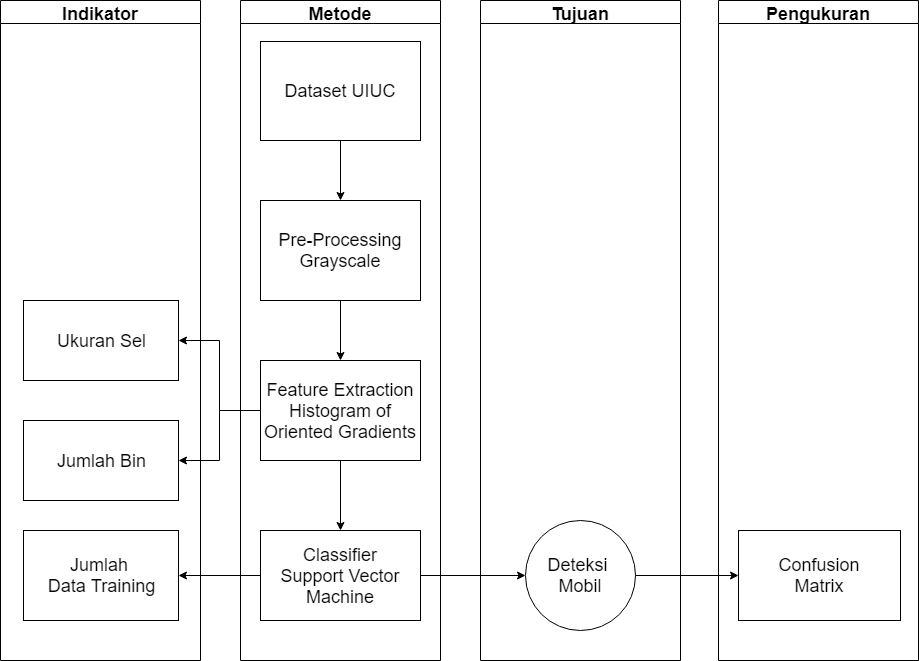
\includegraphics[width=14cm]{images/KerangkaPemikiran.png}}
	\captionof{figure}{Kerangka Pemikiran}
	\label{fig:KerangkaPemikiran}
\end{minipage}
\end{adjustbox}

Berdasarkan gambar \ref{fig:KerangkaPemikiran}, terdapat beberapa variabel indikator yang memengaruhi hasil dan perlu dilakukan penyesuaian meliputi ukuran sel, jumlah \textit{bin} yang menentukan batasan sudut yang digunakan, dan jumlah data \textit{training} untuk \textit{classifier} \textit{Support Vector Machine}. Ukuran sel akan mempengaruhi jumlah fitur. Semakin kecil ukuran sel, jumlah fitur akan bertambah. Penelitian ini bertujuan untuk melihat hasil akurasi dari deteksi mobil menggunakan \textit{confusion matrix}.\\

\section{Urutan Proses Global}
Dalam sistem pengenalan mobilterbagi atas dua proses yaitu proses \textit{training} dan proses \textit{testing}. Proses \textit{training} dilakukan untuk mendapatkan kelas dari objek yang akan dikenali. Proses \textit{testing} dilakukan untuk menghitung hasil yang berupa akurasi dari pengenalan mobil.

\begin{adjustbox}{width=1\textwidth}
	\begin{minipage}{\linewidth}
		\framebox[\textwidth]{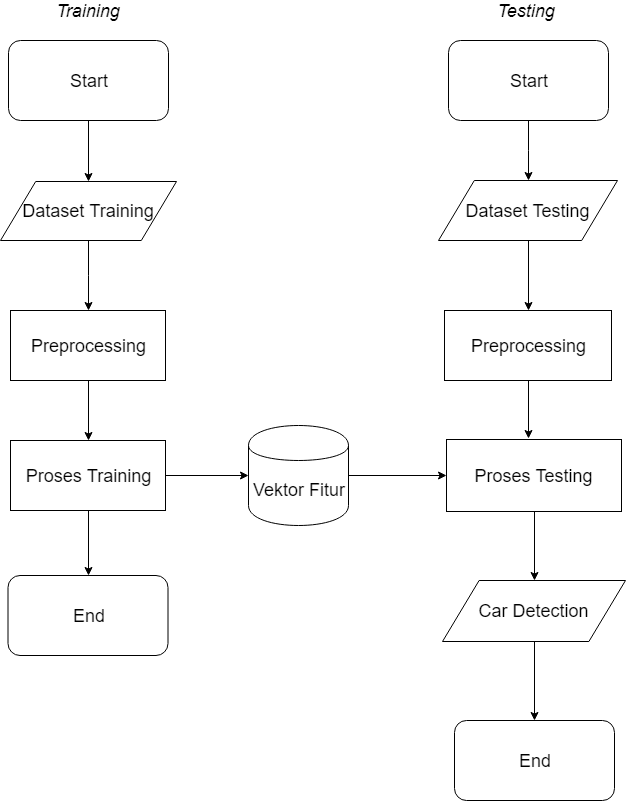
\includegraphics[width=10cm]{images/FlowchartGlobal.png}}
		\captionof{figure}{\textit{Flowchart Global} Sistem Pengenalan Mobil\\}
		\label{fig:FlowchartGlobal}
	\end{minipage}
\end{adjustbox}

Pada gambar \ref{fig:FlowchartGlobal}, dataset yang digunakan akan melalui tahap preprocessing untuk mempermudah proses ekstraksi fitur. Citra tersebut kemudian akan dibagi menjadi data latih dan data uji. Proses pelatihan akan menggunakan data latih untuk memperoleh fitur. Sedangkan proses pengujian akan menggunakan data uji dan fitur yang diperoleh dari tahap pelatihan. Hasil dari tahap pengujian adalah hasil deteksi mobil yang dibuat oleh sistem.
\\

\subsection{Proses \textit{Training}}

\begin{adjustbox}{width=1\textwidth}
	\begin{minipage}{\linewidth}
		\framebox[\textwidth]{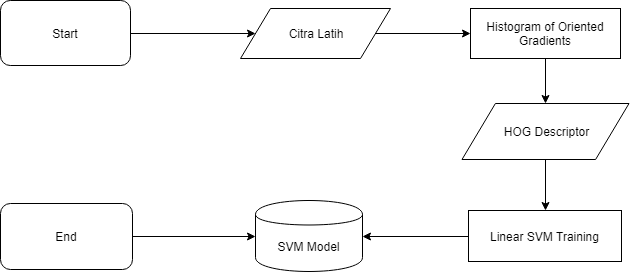
\includegraphics[width=14cm]{images/FlowchartTraining.png}}
		\captionof{figure}{\textit{Flowchart Training} Sistem Pengenalan Mobil\\}
		\label{fig:FlowchartTraining}
	\end{minipage}
\end{adjustbox}

Berikut ini adalah uraian dari \textit{flowchart} pada gambar \ref{fig:FlowchartTraining} yang dilakukan dalam penelitian ini:
\begin{enumerate}
\item Citra yang menjadi masukan yaitu dari data latih yang berisi kumpulan mobil. Citra mobil memiliki ukuran beragam dengan rentang ukuran lebar 200 - 300 piksel dan tinggi 100 - 200 piksel. Citra berupa \textit{grayscale} dengan arah pengambilan citra terdiri dari belakang.
\item \textit{Histogram of Oriented Gradient} berfungsi untuk mengambil fitur dari dari citra masukan. Hasil dari ekstraksi fitur menggunakan HOG adalah \textit{HOG descriptor}.\textit{HOG descriptor} mendeskripsikan distribusi dari gradien berarah pada suatu area citra.
\item Berdasarkan penelitian yang dilakukan oleh Dalal dan Triggs \cite{dalal}, \textit{HOG} menggunakan ukuran sel 8 $\times$ 8 piksel dan 16 $\times$ 16 piksel untuk ukuran blok kemudian \textit{bin} yang digunakan pada tahap pembuatan \textit{histogram} adalah 9 (dimulai dari 0 derajat hingga 180 derajat).
\item \textit{Support Vector Machine} (SVM) digunakan untuk klasifikasi fitur ke dalam 2 kelas (mobil dan bukan mobil) berdasar fitur yang sudah didapatkan. Hasil dari klasifikasi ini nantinya akan disimpan ke dalam bentuk berkas.\\
\end{enumerate}

\subsection{Proses \textit{Testing}}

\begin{adjustbox}{width=1\textwidth}
	\begin{minipage}{\linewidth}
		\framebox[\textwidth]{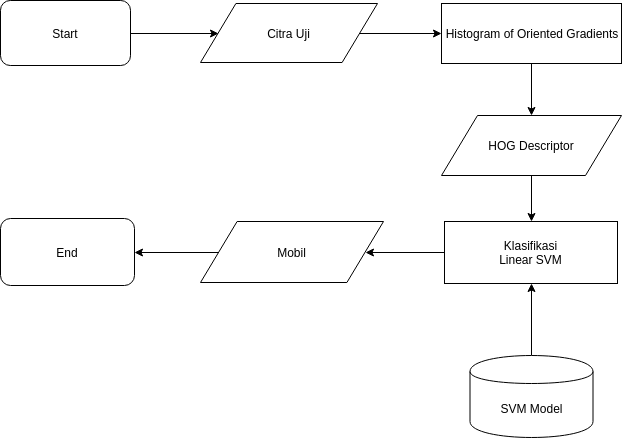
\includegraphics[width=14cm]{images/FlowchartTesting.png}}
		\captionof{figure}{\textit{Flowchart Testing} Sistem Pendeteksi Mobil\\}
		\label{fig:FlowchartTesting}
	\end{minipage}
\end{adjustbox}

\noindent Pada gambar \ref{fig:FlowchartTesting} terlihat alur proses \textit{testing}. Pada proses \textit{testing} terdapat beberapa proses yang sama seperti pada proses \textit{training}. Berikut adalah uraian dari \textit{flowchart} pada gambar \ref{fig:FlowchartTesting} yang dilakukan dalam penelitian ini:
\begin{enumerate}
\item Citra pengujian yang digunakan didapatkan dari \textit{dataset} dan \textit{www.youtube.com}, penggunaan dari dataset ini sesuai dengan perizinan dari institusi yang bersangkutan.
\item Citra yang akan menjadi input dari \textit{HOG} adalah citra hasil dari grayscale citra mobil yang sudah dilakukan pada tahapan \textit{preprocessing}.
\item Ukuran dari sel dan blok yang digunakan untuk proses ekstraksi fitur dengan menggunakan \textit{HOG} adalah sama dengan yang digunakan ketika pada tahap \textit{training}.
\item Pada tahap \textit{testing}, model SVM yang digunakan adalah berkas hasil keluaran dari SVM pada tahap \textit{training}.
\item Hasil keluaran akan berupa penandaan mobil yang berhasil dikenali oleh sistem.\\
\end{enumerate}

\section{Analisis Manual}
Bagian ini melakukan analisis tahapan proses dengan melakukan perhitungan manual. Analisis untuk proses pelatihan dan pembelajaran pada penelitian ini berjumlah yaitu mobil dan bukan mobil.\\

\subsection{\textit{Dataset}}
Dataset yang digunakan terdiri dari 3 jenis data latih yang diambil dari sumber yang berbeda. Penelitian ini menggunakan \textit{dataset UIUC Car Image Database}, \textit{GTI Database}, dan \textit{KITTI Database}. Arah pengambilan kamera untuk \textit{dataset} dilakukan dari posisi \textit{horizontal}.

Dataset \textit{UIUC Car Image Database} diperoleh dari \textit{http://cogcomp.org/Data/Car/}. Citra yang diambil dari \textit{dataset} merupakan citra \textit{grayscale} dengan 8 channel warna. Pada UIUC terdapat 1328 citra mobil. Dari total \textit{dataset} yang digunakan, terdiri dari 1050 citra latih dan 278 citra uji. Citra latih dibagi menjadi 2 macam, yaitu 550 citra mobil dan 500 bukan mobil. Citra mobil yang digunakan untuk citra latih diambil dari 2 arah yaitu kiri dan kanan. Citra uji terdiri dari beragam citra mobil yang terdiri dari 2 jenis yaitu 170 citra \textit{single-scale} dan 108 citra \textit{multi-scale} dengan ukuran panjang berkisar 100 piksel sampai 300 piksel dan lebar 75 piksel sampai 180 piksel. Pembagian data untuk pelatihan dan pengujian sudah dilakukan dari sumbernya. 

\begin{table}[H]
	\small
	\begin{adjustbox}{width=1\textwidth}
		\begin{tabular}{| p {14cm} |}
			\hline
			\begin{figure}[H]
				\centering
				\subfloat[ ]{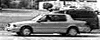
\includegraphics[width = 7cm]{images/DatasetUIUCLatihMobilKiri}} 
				\subfloat[ ]{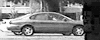
\includegraphics[width = 7cm]{images/DatasetUIUCLatihMobilKanan}} \\
				\subfloat[ ]{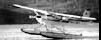
\includegraphics[width = 7cm]{images/DatasetUIUCLatihBukanMobil}}
				\subfloat[ ]{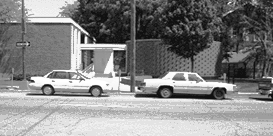
\includegraphics[width = 7cm]{images/DatasetUIUCUji}}\\
			\end{figure} \\
			\hline
		\end{tabular}
	\end{adjustbox}
	\captionof{figure}{Contoh \textit{Dataset UIUC}. (a) Data Latih Mobil (Kiri) (b) Data Latih Mobil (Kanan) (c) Data Latih Bukan Mobil (d) Data Uji}
	\label{fig:ContohUIUC}
\end{table}

\textit{Dataset GTI Database} diperoleh dari \textit{http://www.gti.ssr.upm.es/data/Vehicle\_database.html}. Citra yang diambil dari \textit{dataset} merupakan citra RGB dengan 24 channel warna. Untuk proses pelatihan dan pengujian, ada total 2826 data citra. Data latih yang digunakan diambil dari belakang mobil dengan 3 sudut pengambilan yaitu belakang lurus, belakang kiri, dan belakang kanan. Pengambilan citra dari belakang dilakukan dengan jarak dekat dan jarak jauh. Pembagian data untuk pelatihan dan pengujian dilakukan manual oleh peneliti.

\begin{table}[H]
	\small
	\begin{adjustbox}{width=1\textwidth}
		\begin{tabular}{| p {14cm} |}
			\hline
		\begin{figure}[H]
			\centering
			\subfloat[ ]{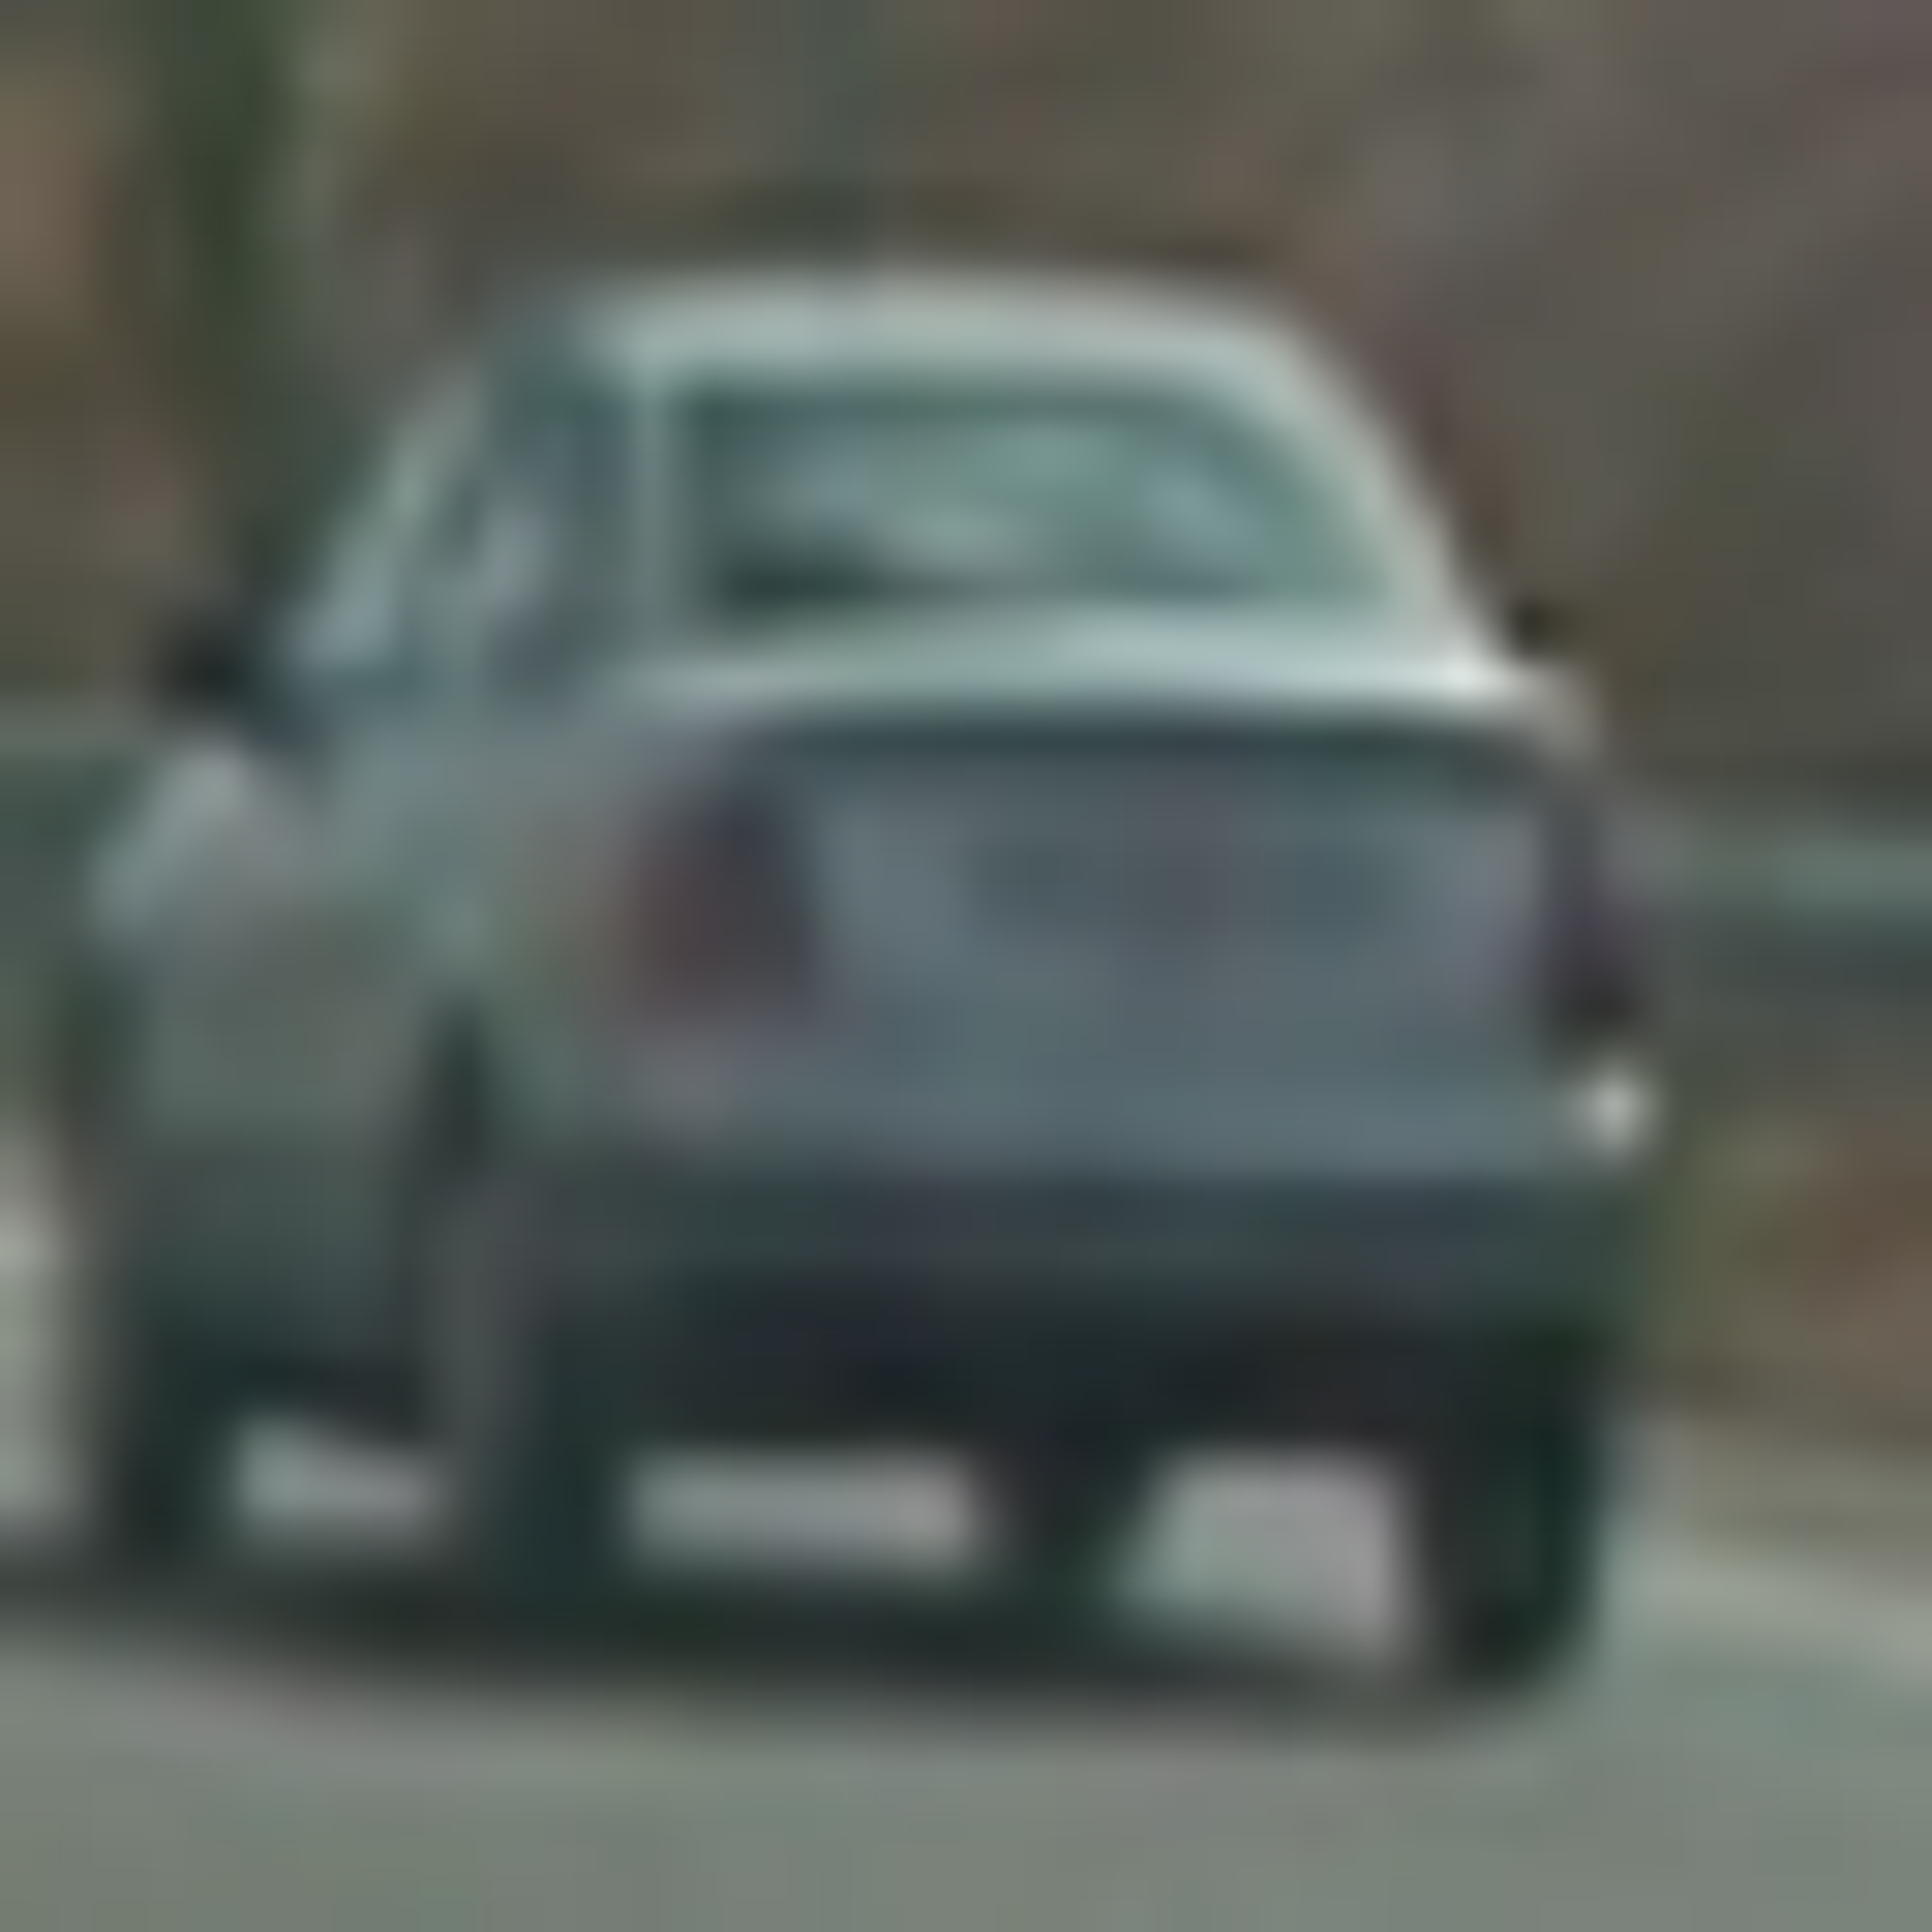
\includegraphics[width = 7cm]{images/DatasetGTILatihMobilKanan}}
			\subfloat[ ]{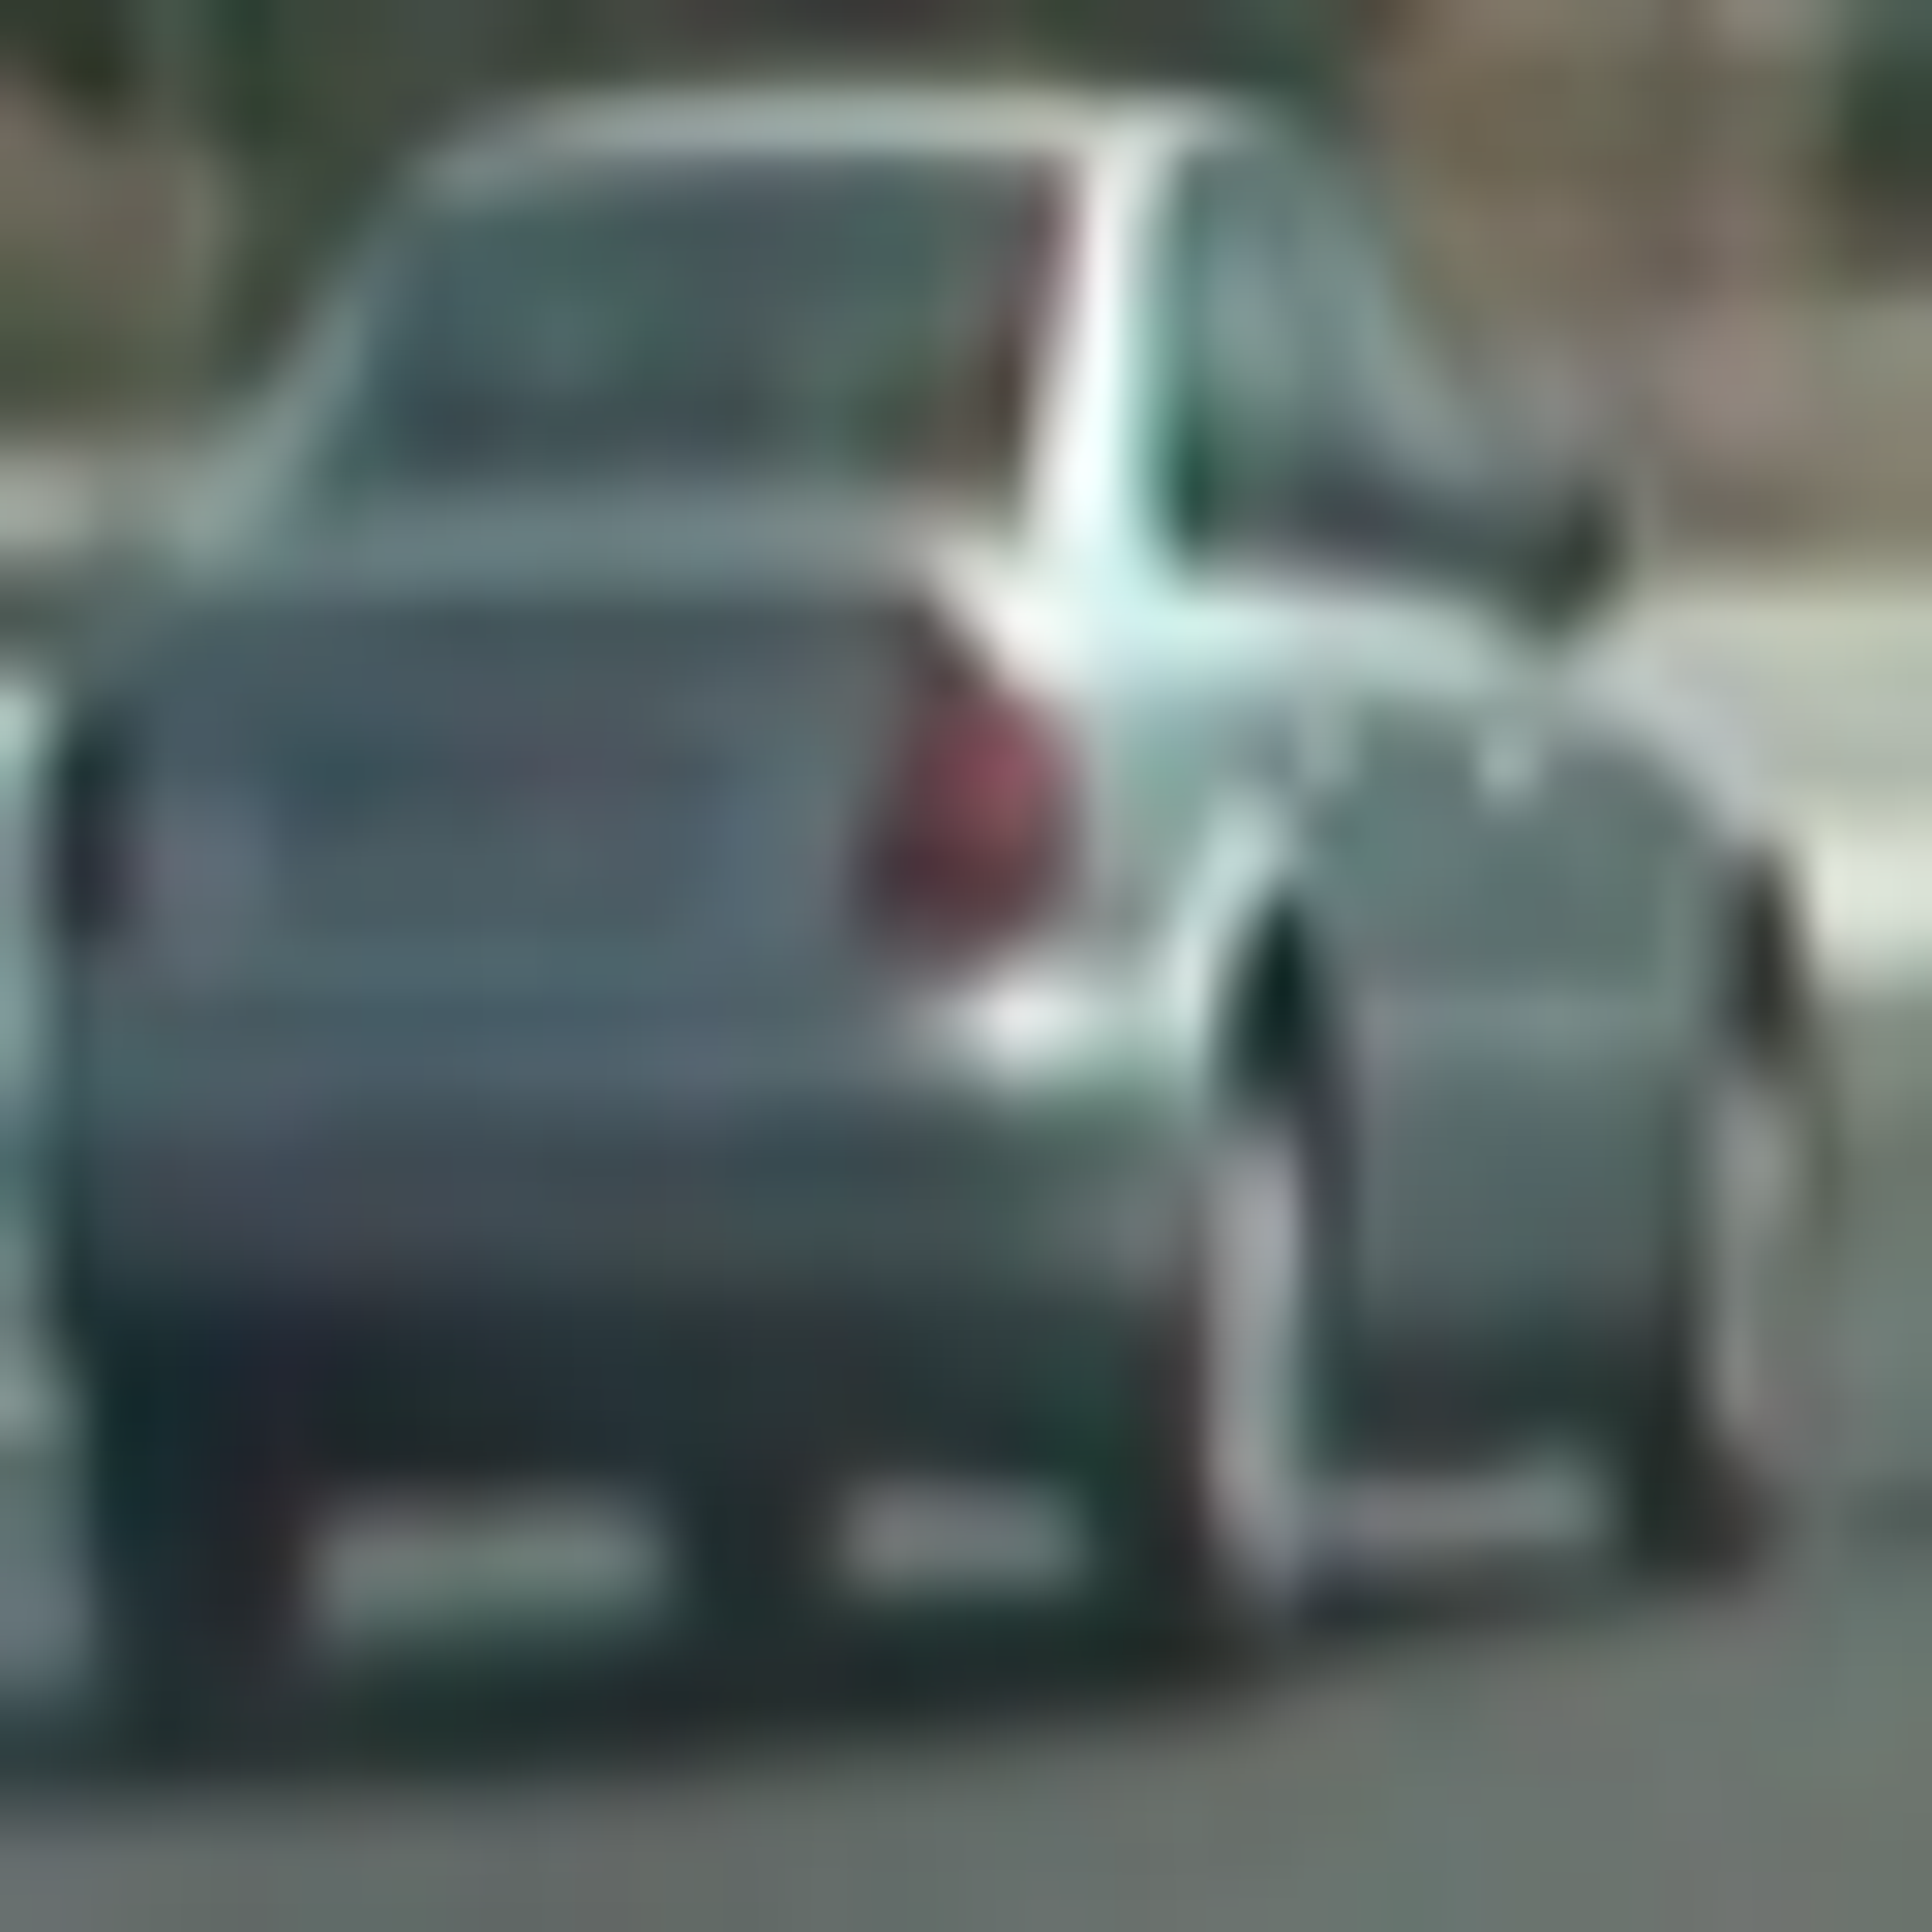
\includegraphics[width = 7cm]{images/DatasetGTILatihMobilKiri}}\\
			\subfloat[ ]{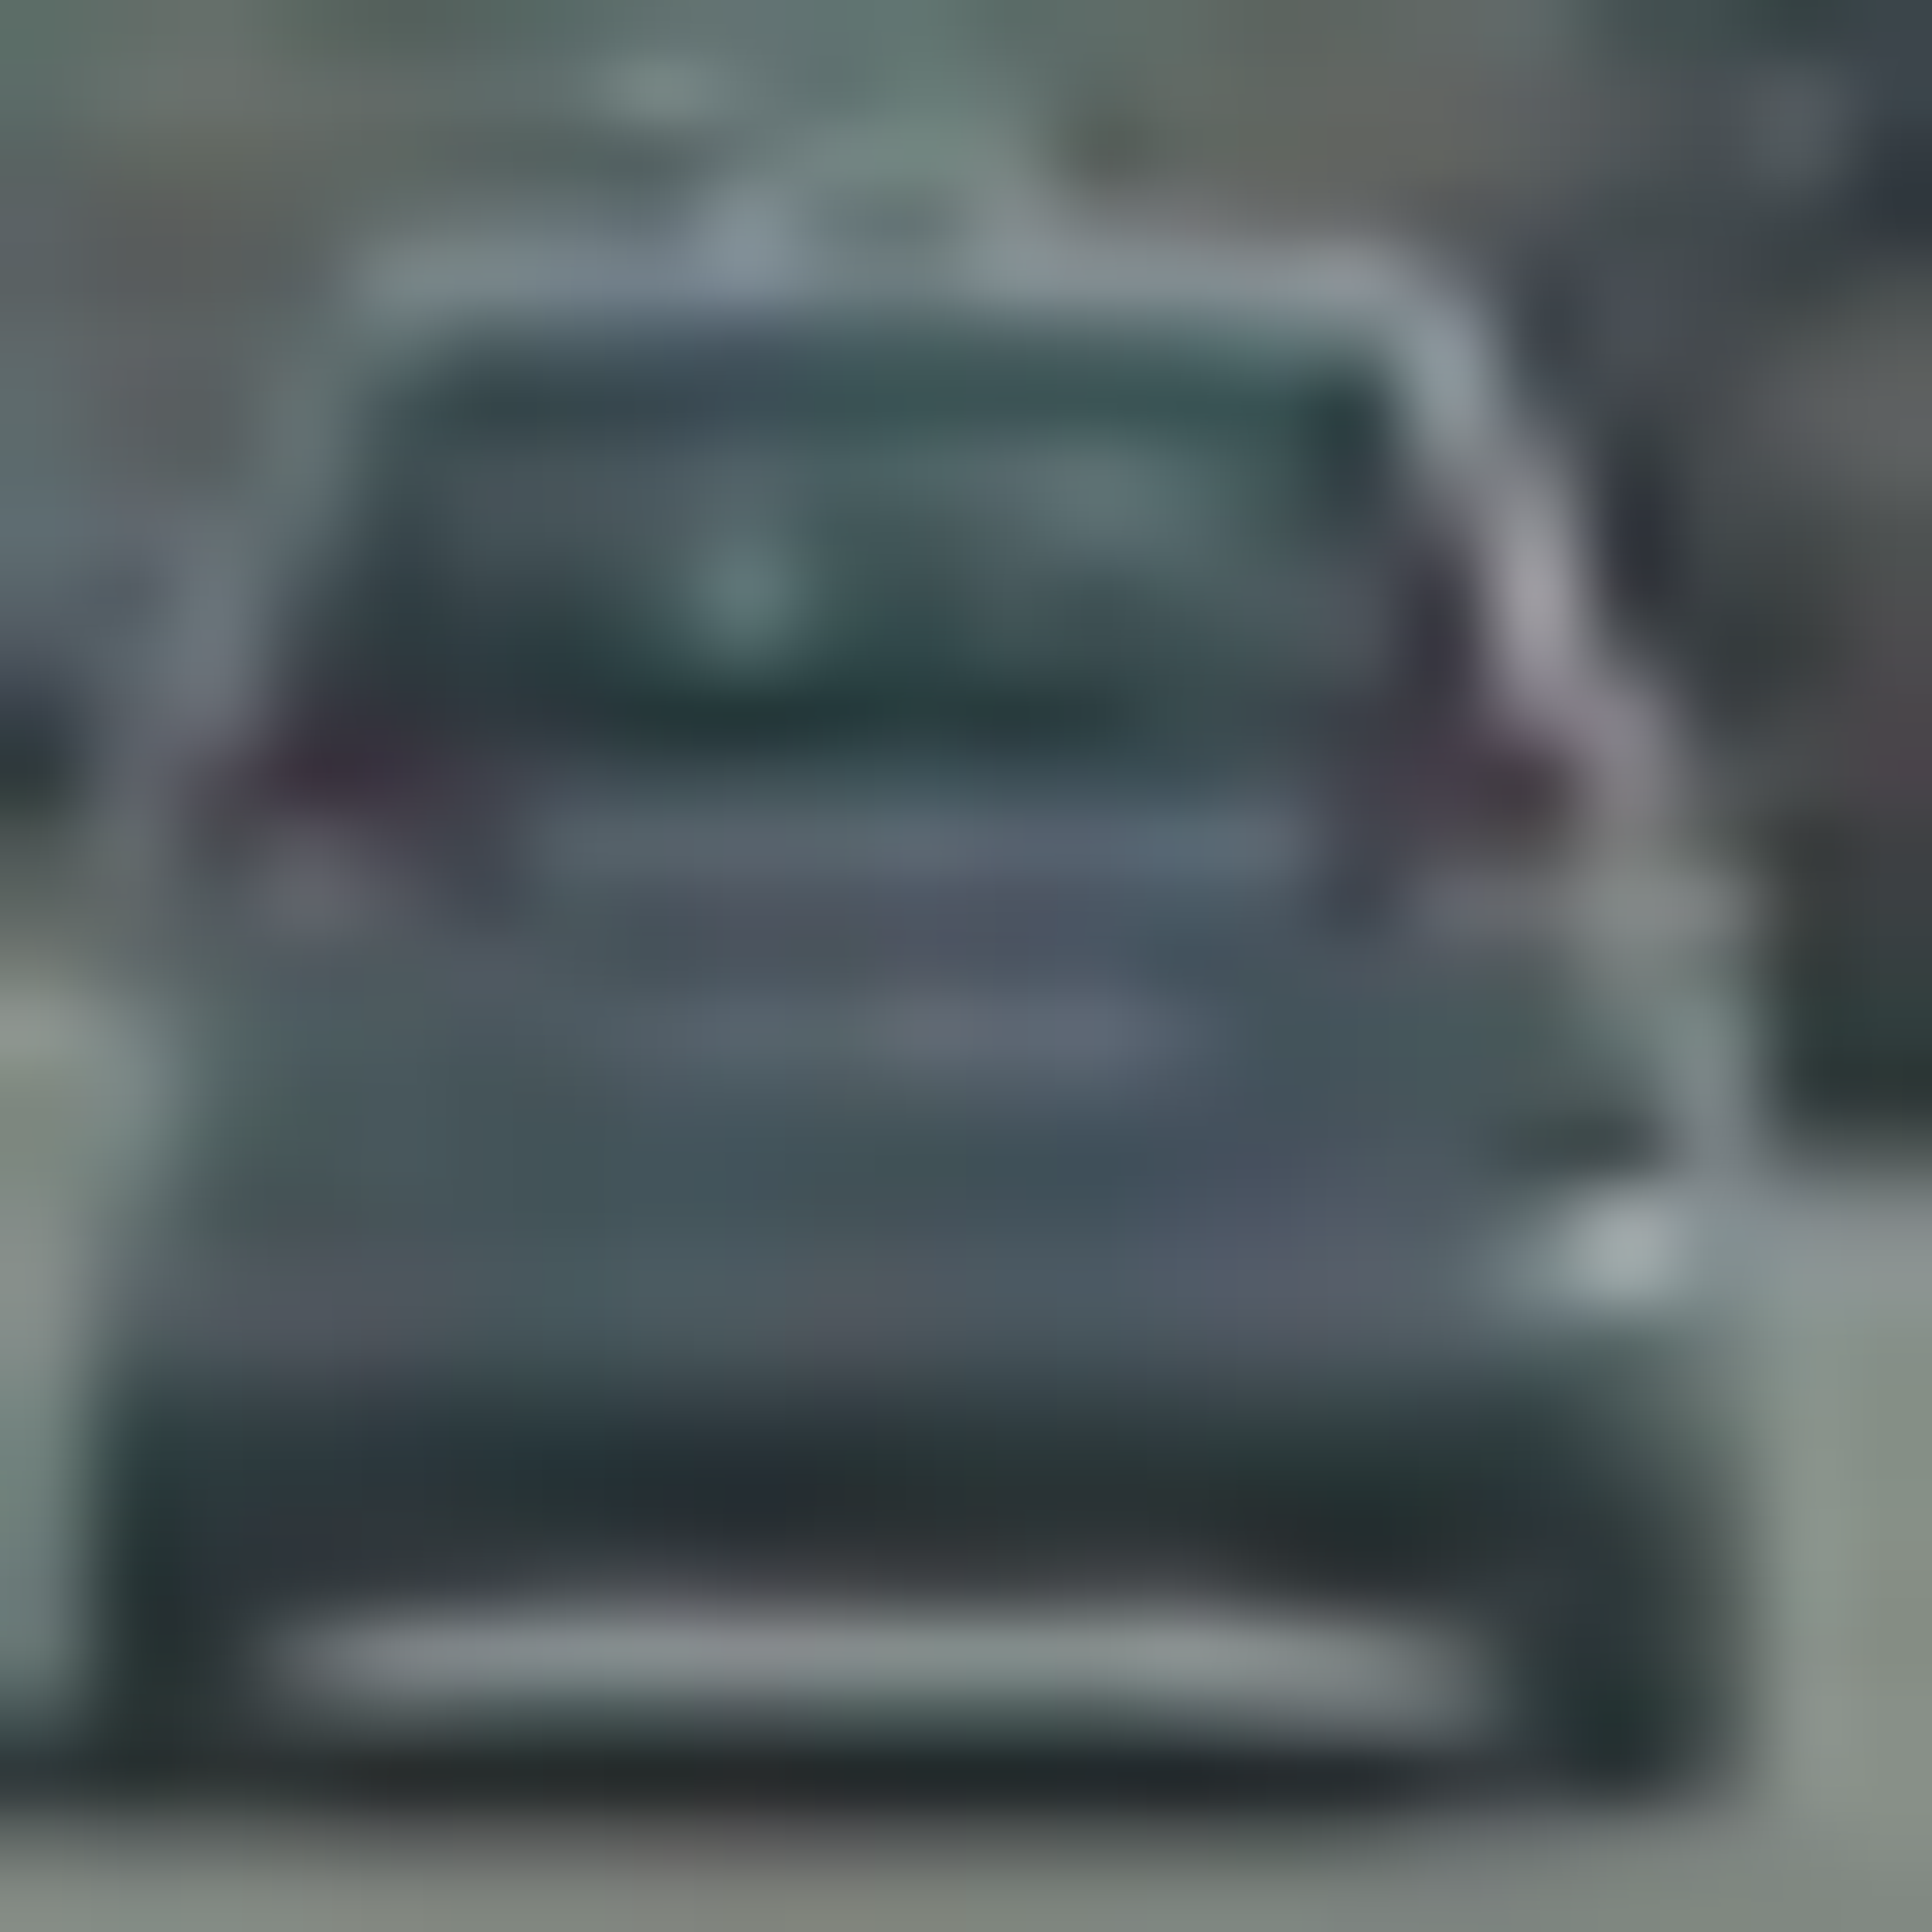
\includegraphics[width = 7cm]{images/DatasetGTILatihMobilJauh}}
			\subfloat[ ]{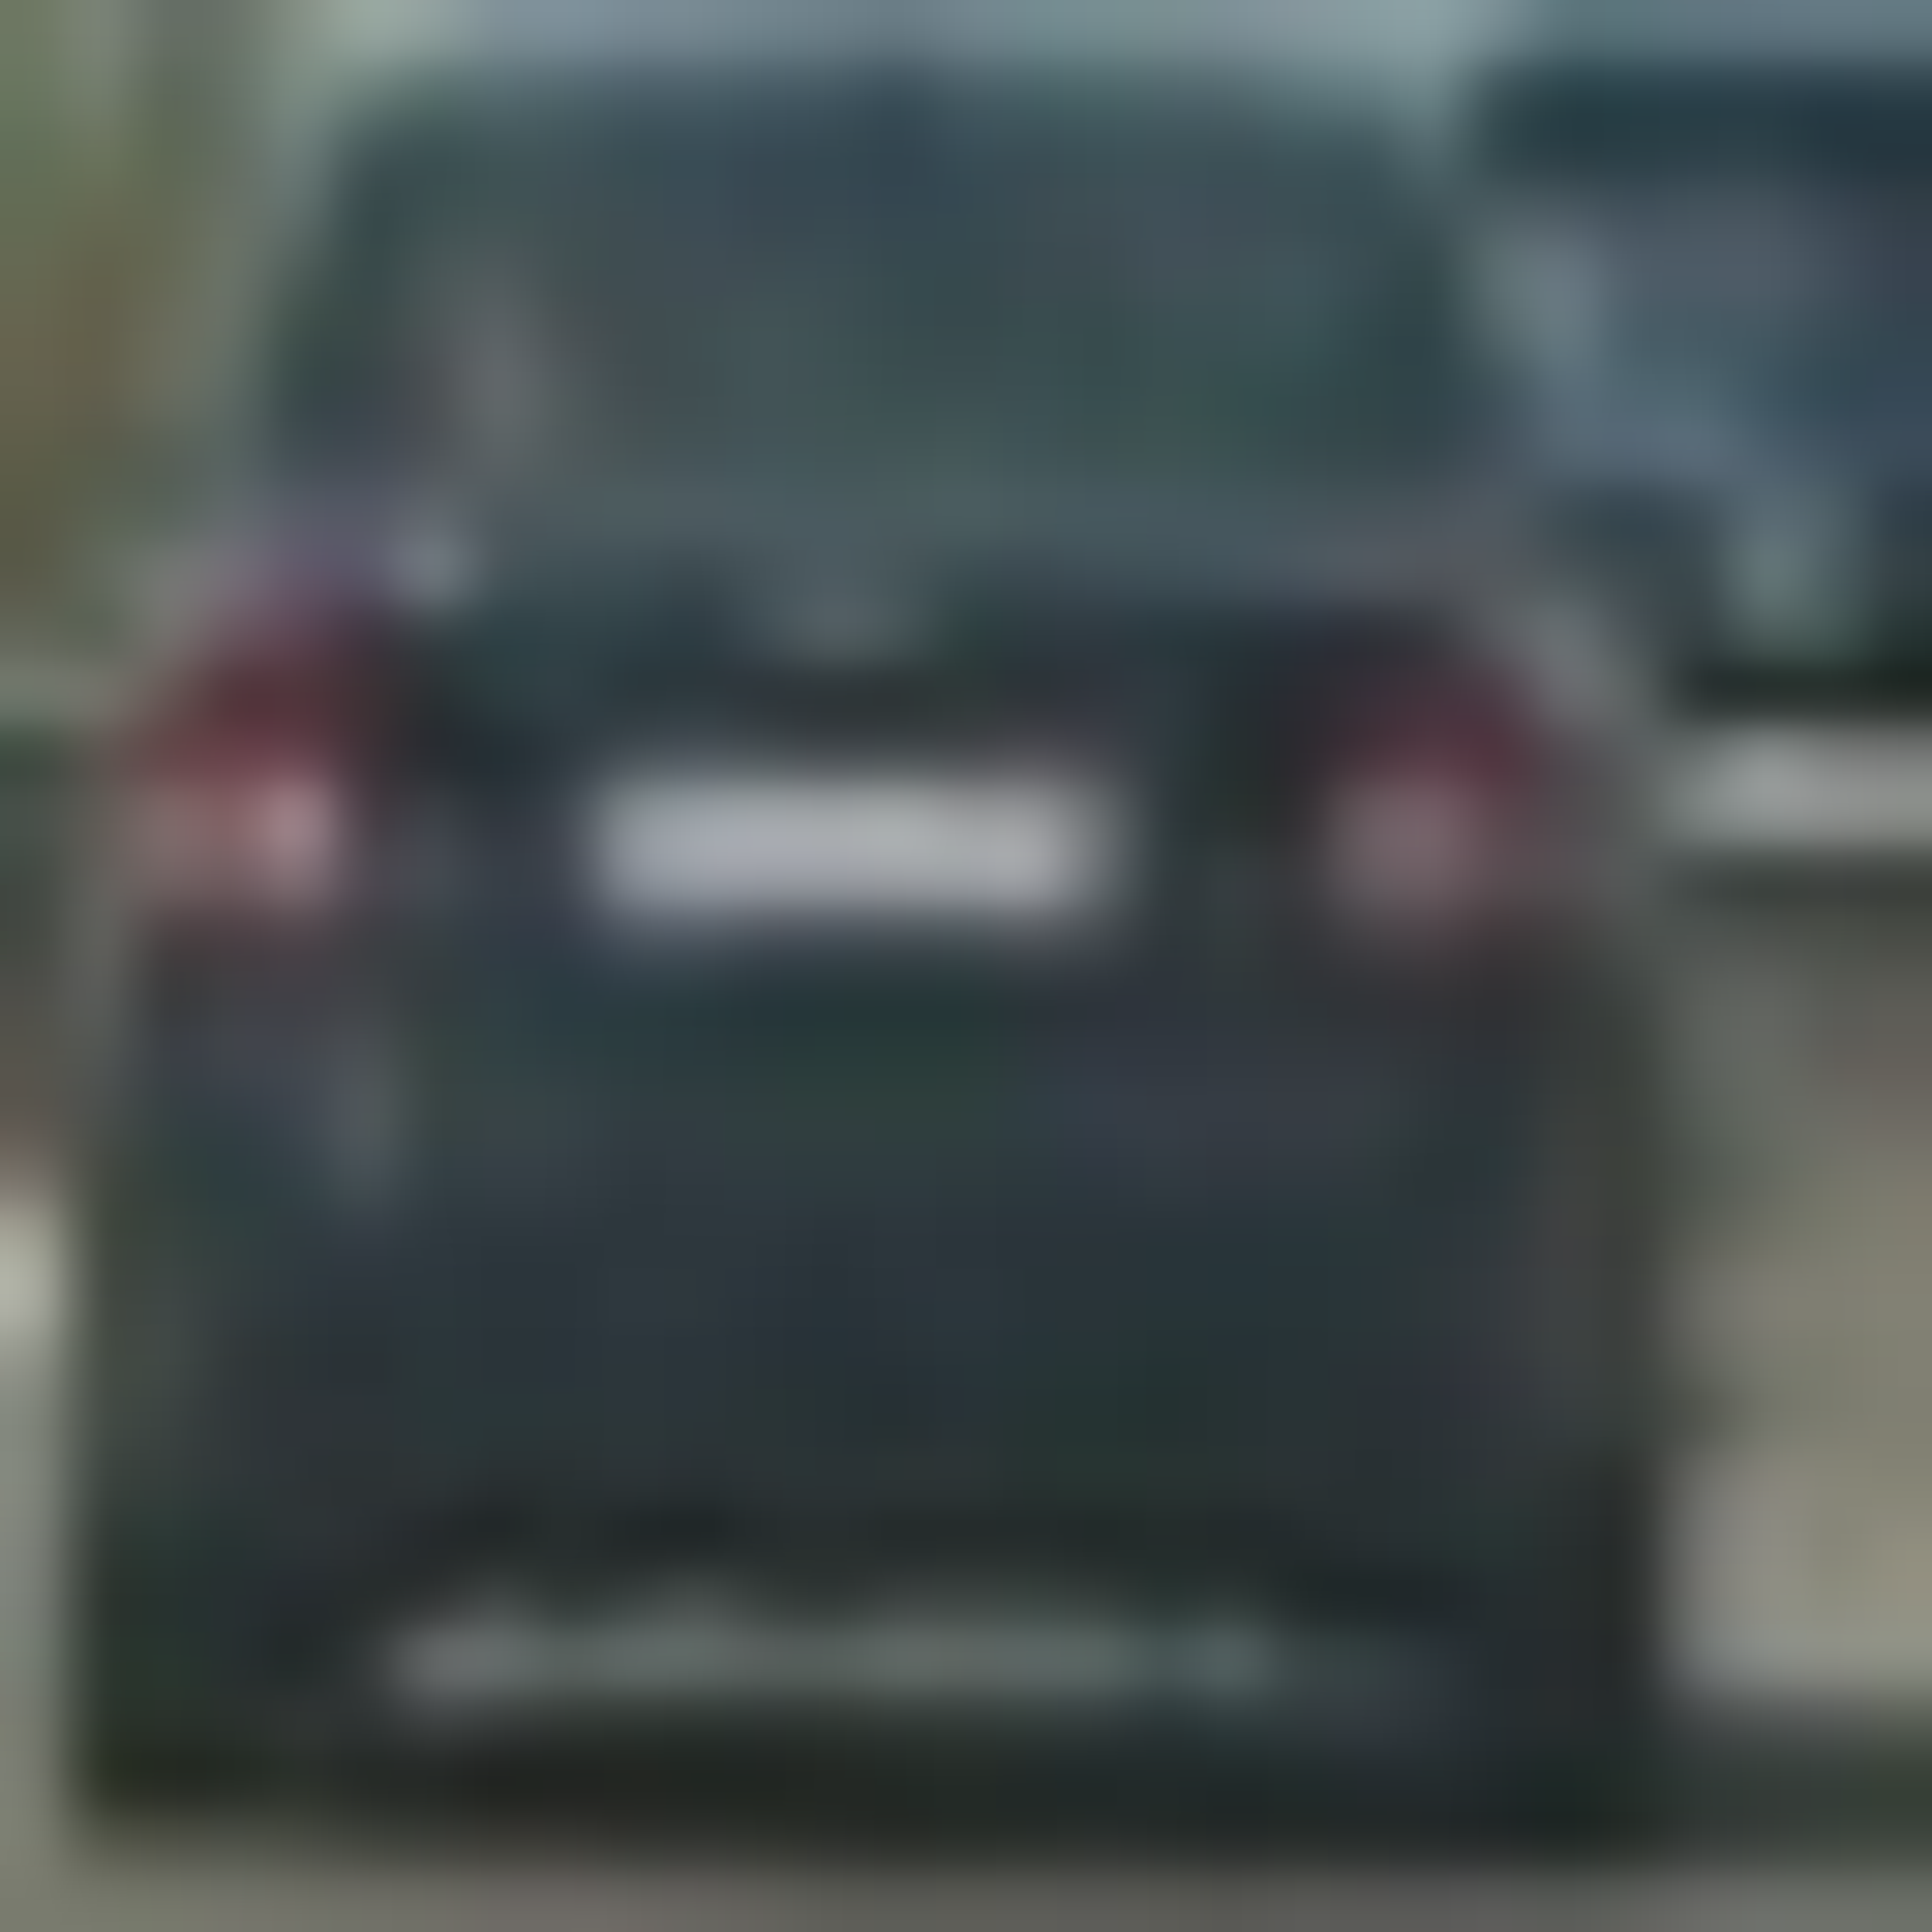
\includegraphics[width = 7cm]{images/DatasetGTILatihMobilDekat}}\\
			\subfloat[ ]{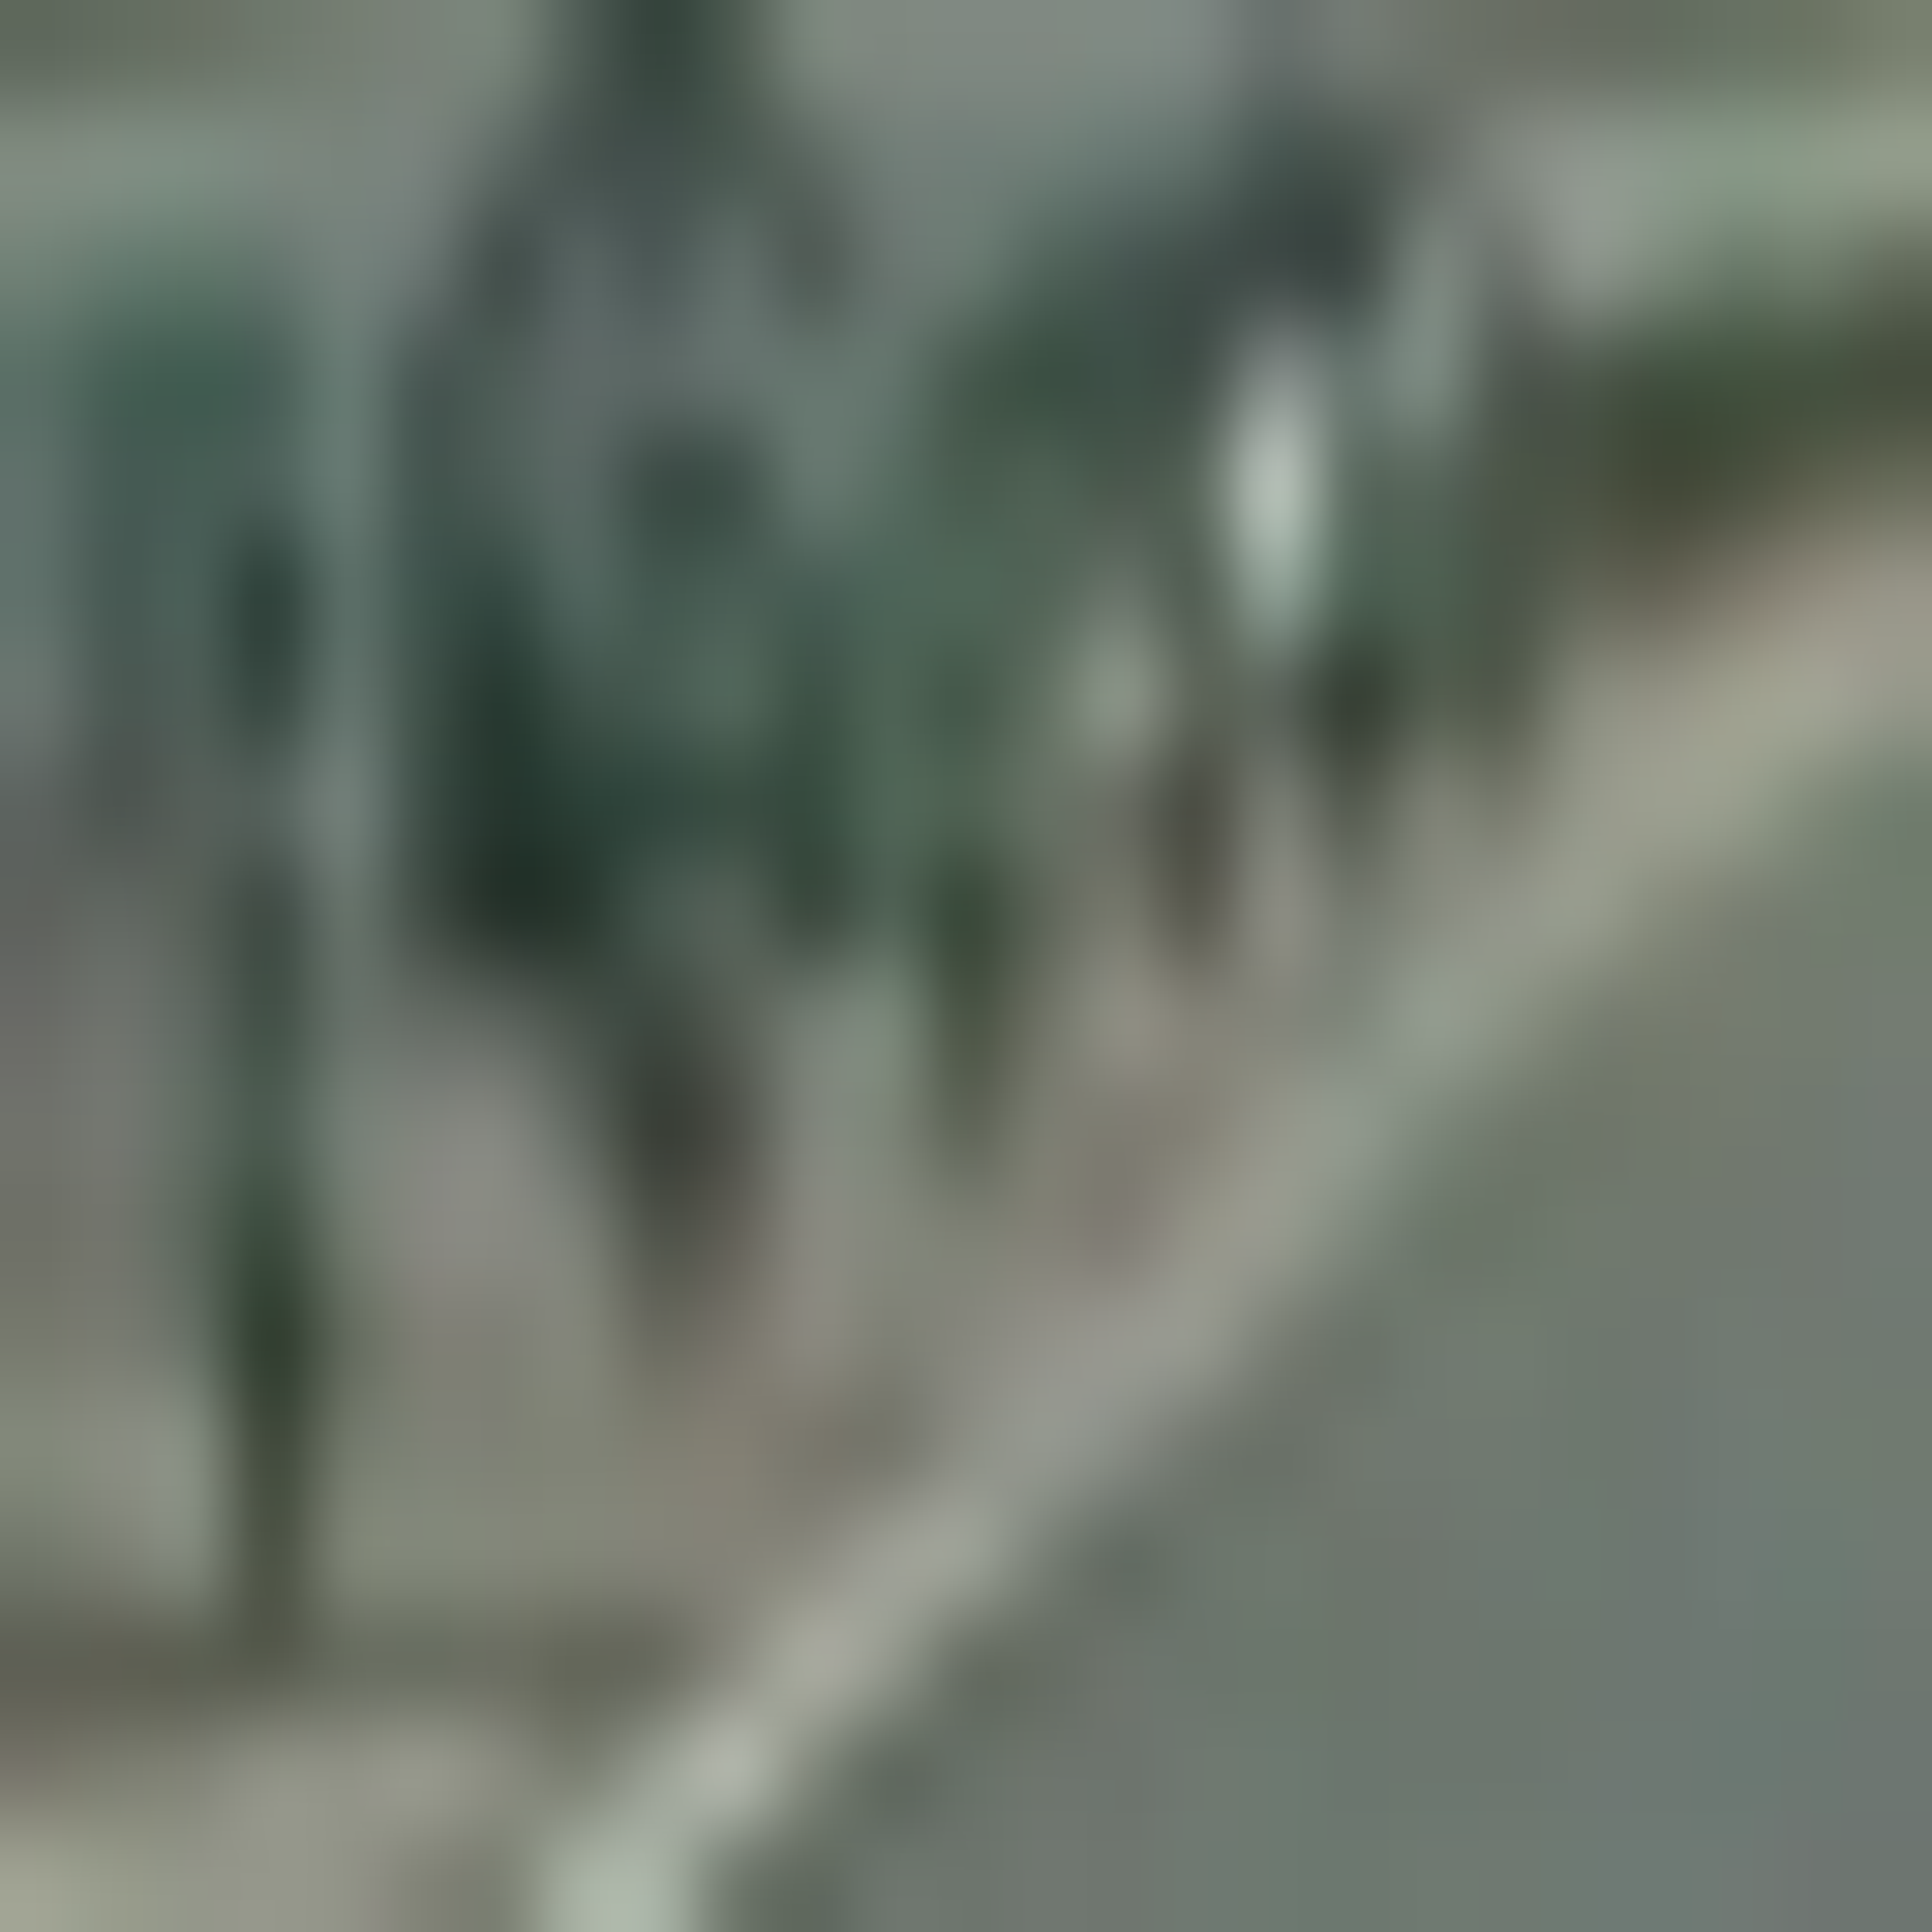
\includegraphics[width = 7cm]{images/DatasetGTILatihBukanMobil}}
			\subfloat[ ]{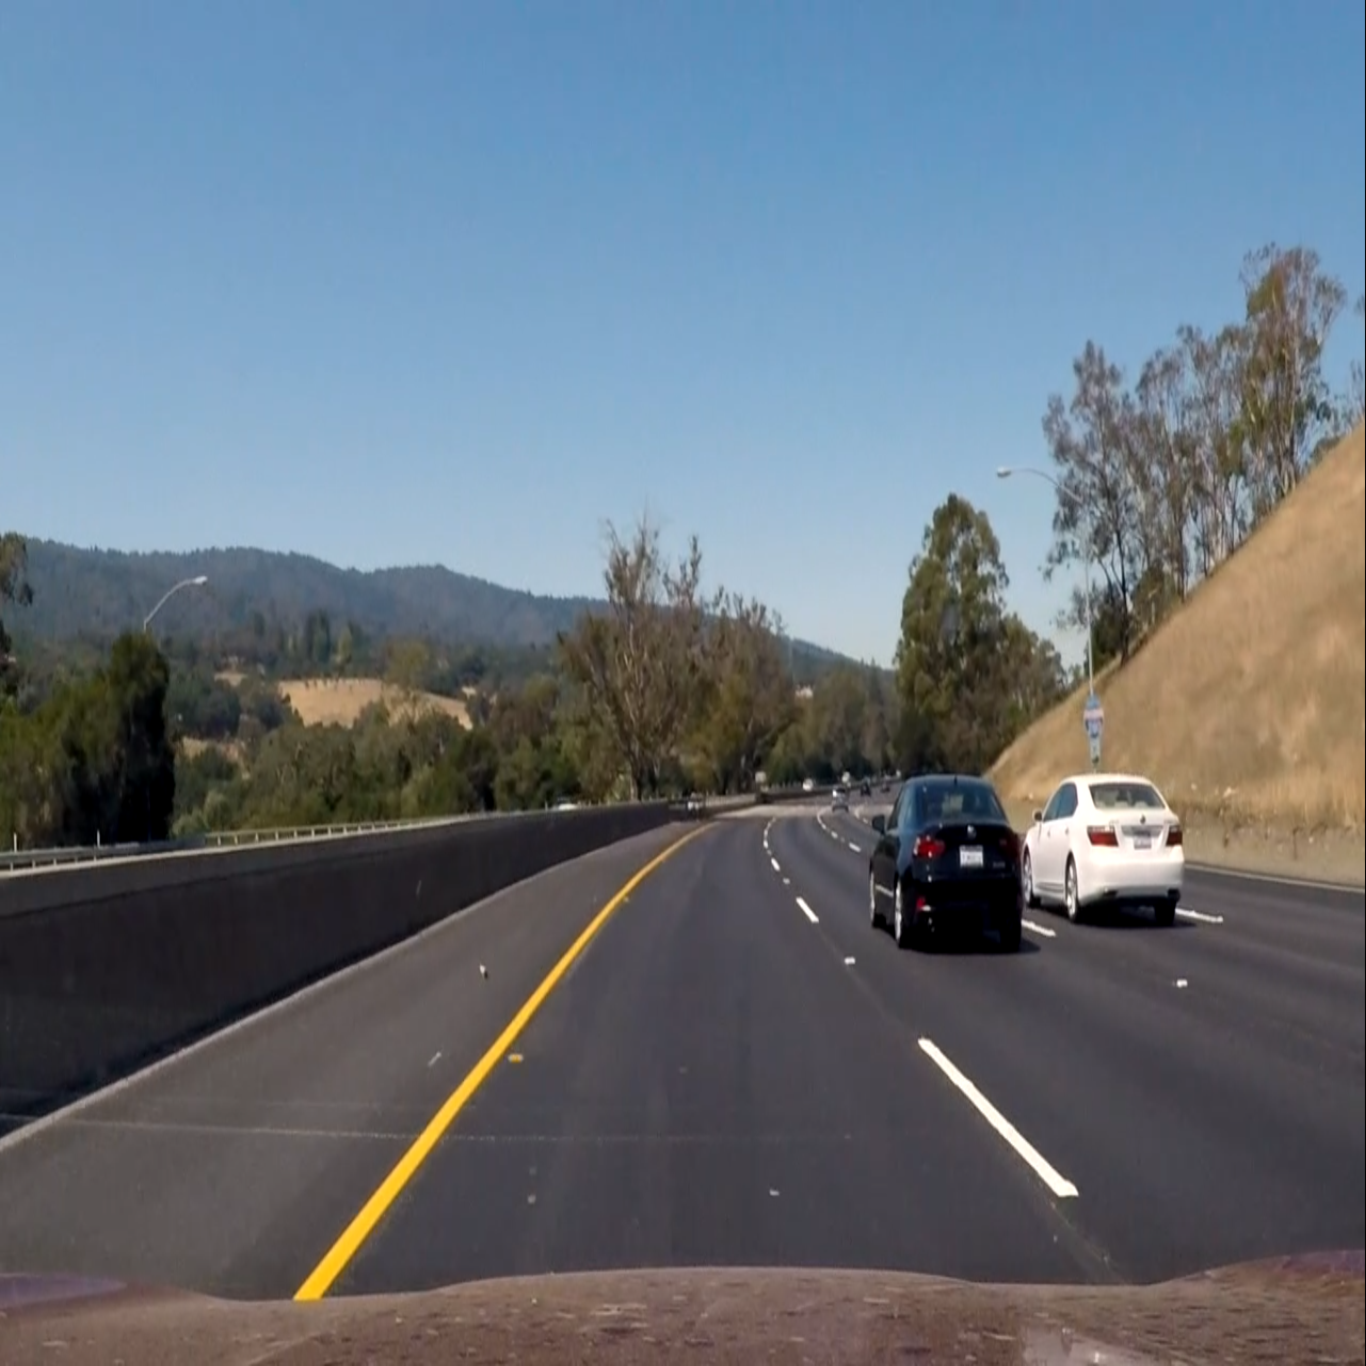
\includegraphics[width = 7cm]{images/DatasetGTIUji}}\\
		\end{figure} \\
			\hline
		\end{tabular}
	\end{adjustbox}
	\captionof{figure}{Contoh \textit{Dataset GTI}. (a) Data Latih Mobil (kiri) (b) Data Latih Mobil (kanan) (c) Data Latih Mobil (jauh) (d) Data Latih Mobil (dekat) (e) Data Latih Bukan Mobil (f) Data Uji}
	\label{fig:ContohGTI}
\end{table}

\textit{Dataset KITTI Database} diperoleh dari \textit{http://www.cvlibs.net/datasets/kitti/}. \textit{Dataset KITTI} merupkan data latih yang berupa mobil yang sama dengan GTI, namun dengan kondisi pencahayaan dan arah yang berbeda. Citra yang diambil dari \textit{dataset} merupakan citra RGB dengan 24 channel warna. Untuk proses pelatihan, ada total 5966 data citra yang diambil dari \textit{dataset}.

\begin{table}[H]
	\small
	\begin{adjustbox}{width=1\textwidth}
		\begin{tabular}{| p {14cm} |}
			\hline
			\begin{figure}[H]
				\centering
				{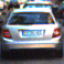
\includegraphics[width = 5cm]{images/DatasetKITTILatihMobil}}
				{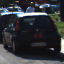
\includegraphics[width = 5cm]{images/DatasetKITTILatihMobil1}}
				{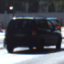
\includegraphics[width = 5cm]{images/DatasetKITTILatihMobil2}}
			\end{figure} \\
			\hline
		\end{tabular}
	\end{adjustbox}
	\captionof{figure}{Contoh \textit{Dataset KITTI}, data data latih mobil}
	\label{fig:ContohKITTI}
\end{table}

Ukuran setiap data latih akan diubah menjadi berukuran 64 x 64 piksel. Format citra dari \textit{dataset} ini akan diubah \textit{Portable Gray Map} (PGM) dengan 8 bit kedalaman \textit{depth}. Data latih dibagi menjadi 2 jenis yaitu mobil (kondisi utuh, tidak ada bagian mobil yang terpotong) dan bukan mobil (jalanan, motor, rumah, pejalan kaki, dan sebagainya). Pembagian data latih terdiri dari 4 jenis pengambilan citra, yaitu jauh, dekat, kiri, dan kanan.

Untuk citra uji, terdiri dari mobil yang berbeda - beda. Citra data uji diambil dari \textit{www.youtube.com} yang akan diproses secara citra digital. Dari video akan diambil beberapa frame untuk dideteksi keberadaan mobil. Ukuran untuk setiap citra uji beragam dengan panjang antara 110 piksel sampai 301 piksel dan lebar 75 piksel sampai 179 piksel dengan \textit{depth bit} 24.

Pada dataset juga terdapat \textit{template} untuk \textit{Region of Interest} dimana berupa citra biner yang berfungsi untuk menandai lokasi dimana mobil akan melaju. ROI digunakan pada saat proses \textit{testing}. Penggunaan ROI ditandai dengan nilai 1 untuk \textit{foreground} dan 0 untuk \textit{background}.

\begin{table}[H]
	\small
	\begin{adjustbox}{width=1\textwidth}
		\begin{tabular}{| p {14cm} |}
			\hline
			\begin{figure}[H]
				\centering
				{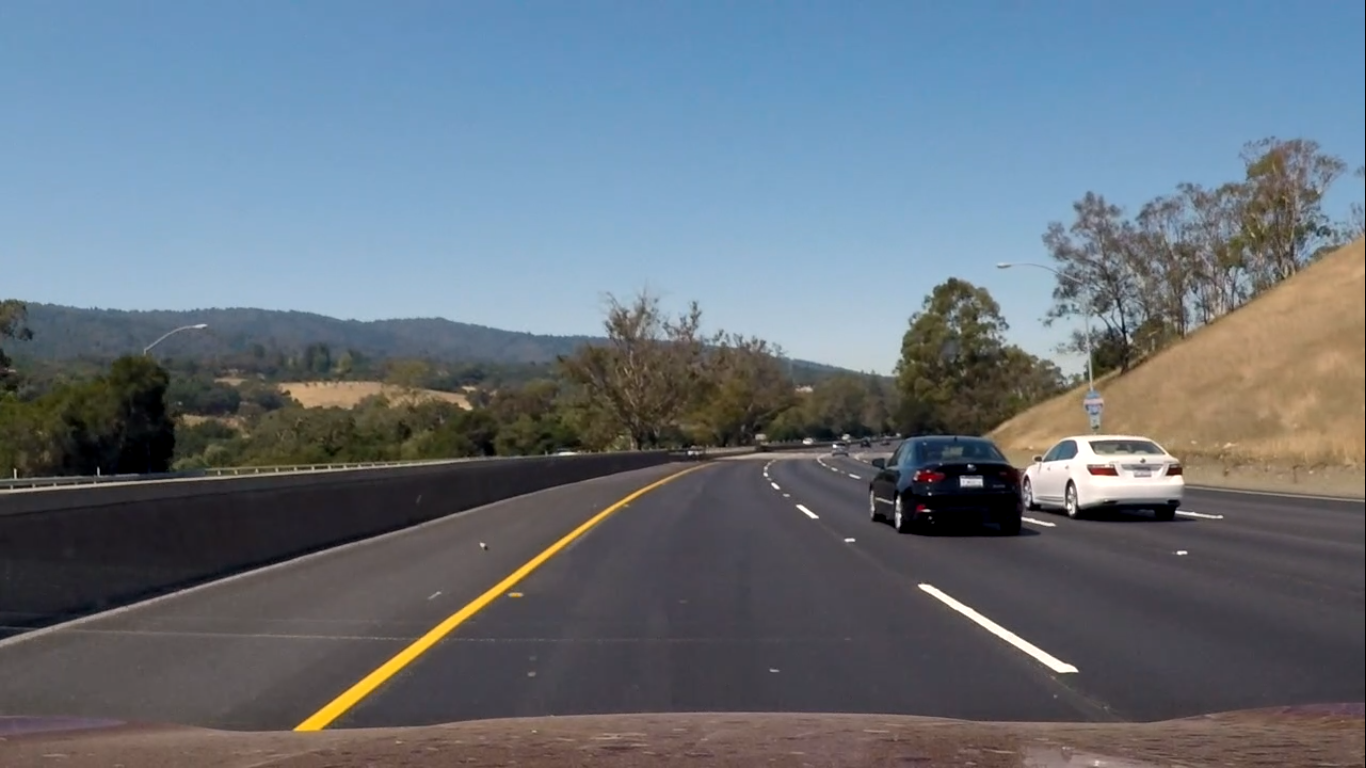
\includegraphics[height = 4cm]{images/ROI}} 
				{
\includegraphics[height = 4cm]{images/ROI_biner}}\\
			\end{figure} \\
			\hline
		\end{tabular}
	\end{adjustbox}
	\captionof{figure}{Contoh ROI}
	\label{fig:ContohROI}
\end{table}

Analisis selanjutnya akan dilakukan untuk menangani kasus dimana bagian dari mobil yang terdapat dalam citra uji hanya sebagian, terdapat lebih dari 1 mobil dalam 1 citra uji, dan ukuran objek berdasar jarak kamera dengan objek penelitian (mobil). Mobil yang akan terdeteksi memiliki ukuran terkecil 64 x 64 piksel.
\\

\subsection{Tahap Pendeteksian Lokasi Mobil}
Seperti dijelaskan sebelumnya, sistem pendeteksian mobil terdiri dari beberapa tahap. Citra input pertama - tama dibuat menjadi \textit{grayscale}, kemudian melalui tahap ekstraksi fitur dengan \textit{Histogram of Oriented Gradients}, dan terakhir fitur yang diperoleh kemudian diklasifikasi dengan \textit{Support Vector Machines}. Berikut adalah skema alur dari tahap pendeteksian lokasi mobil.
\\

\subsubsection{\textit{Grayscale}}
Proses pertama yaitu mengubah citra masukan menjadi citra \textit{grayscale}. Tujuan dari \textit{grayscaling} citra adalah untuk menghilangkan informasi warna dari setiap piksel citra. Dalam proses deteksi mobil dengan HOG, input warna tidak diperlukan karena warna tidak diperlukan oleh metode HOG. Di bawah merupakan contoh matriks citra asli dengan 3 \textit{channel} warna yaitu \textit{Red}, \textit{Green}, dan \textit{Blue} berukuran 5 $\times$ 5 piksel yang diambil dengan menggunakan \textit{image tools} dari aplikasi \textit{MatLab}. \\

\begin{adjustbox}{width=1\textwidth}
	\begin{minipage}{\linewidth}
		\framebox[\textwidth]{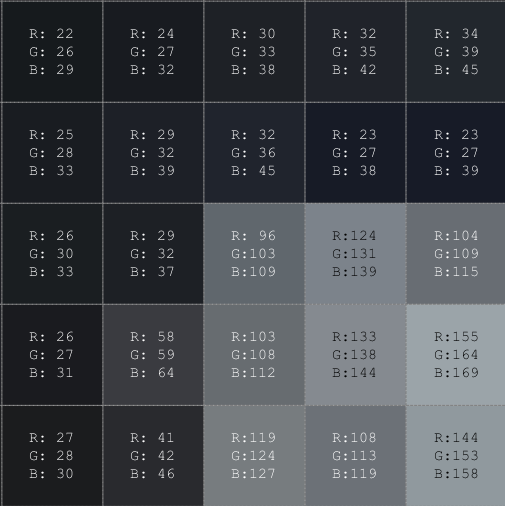
\includegraphics[width=5cm]{images/CitraMatriksAsal.PNG}}
		\captionof{figure}{Matriks Citra Asal berukuran 5 $\times$ 5\\}
		\label{fig:MatriksCitraAsal}
	\end{minipage}
\end{adjustbox} \\

Dari contoh nilai citra RGB di atas, akan diubah menjadi nilai \textit{grayscale} menggunakan rumus \eqref{eq:grayscale} dengan perhitungan sebagai berikut:

\begin{table}[H]
	\begin{adjustbox}{width=1\textwidth}
		\begin{tabular}{|p{13.55cm}|}
			\hline
			\begin{equation}\nonumber
			\begin{aligned}
			Matriks[3,3] &= (0.299 * 133) + (0.587 * 138) + (0.114 * 144) \\
						 &= 137.189 \approx 137 
			\end{aligned}
			\end{equation}\\
			\hline
		\end{tabular}
	\end{adjustbox}
\end{table}

Perhitungan di atas diterapkan pada seluruh piksel pada citra asal yang kemudian menghasilkan matriks citra berukuran 5 $\times$ 5 dengan satu nilai derajat keabuan.

\begin{adjustbox}{width=1\textwidth}
	\noindent\begin{minipage}{\linewidth}
		\framebox[\textwidth]{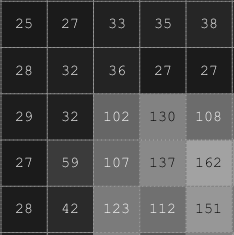
\includegraphics[width=5cm]{images/CitraMatriksGrayscale.PNG}}
		\captionof{figure}{Matriks Citra Hasil Grayscale\\}
		\label{fig:MatriksCitraGrayscale}
	\end{minipage}
\end{adjustbox} \\

\subsection{\textit{Histogram of Oriented Gradient}}
Hasil citra \textit{grayscale} dari \textit{preprocessing} kemudian digunakan untuk input HOG. HOG bertujuan untuk mengambil fitur dari citra masukkan. Hasil dari proses ini adalah vektor fitur yang berbentuk matriks fitur dimana ukurannya ditentukan berdasar jumlah \textit{bin}, ukuran sel dan blok. Ukuran sel, blok, dan jumlah \textit{bin} akan dianalisis pada bab selanjutnya.
%Metode HOG pada penelitian ini dijelaskan melalui \textit{pseudocode} berikut:

\noindent\fbox{\parbox{\textwidth}{\textit{Peseudocode:}
\begin{enumerate}
	\item \textbf{Masukan:} Citra \textit{grayscale} hasil resize.
	\item Menentukan jumlah \textit{bin}, ukuran sel, dan ukuran blok.
	\item Menghitung nilai gradien dan arah gradien untuk setiap piksel dari citra masukan dengan persamaan \ref{eqn:BesarGradien} dan \ref{eqn:ArahGradien}.
	\item Menghitung nilai magnitude gradien dan arah gradien untuk setiap piksel dari citra masukan menggunakan hasil dari tahap 2 sebelumnya.
	\item Membagi citra masukan ke dalam ukuran sel yang sudah ditentukan.
	\item Untuk setiap sel, lakukan proses vote untuk setiap c \textit{bin} terhadap sudutnya dengan menggunakan magnitude gradien dan arah gradien dari tahap 4.
	\item Untuk setiap blok (a x b sel), gabungkan histogram \textit{bin} ke dalam satu matriks baris, sehingga didapat ukuran [a x b x c] x 1 matriks untuk proses normalisasi.
	\item Menggunakan rumus algoritme \textit{L2 Norm} dengan menggunakan persamaan \ref{eqn:normalisasi2} dalam proses normalisasi kemudian lakukan proses normalisasi berupa \textit{sliding window} dengan melakukan pergeseran sebesar ukuran 1 sel ke arah vertikal dan horizontal dari hasil tahap 6.
	\item Untuk setiap hasil normalisasi, gabungkan seluruh matriks baris sehingga membentuk sebuah fitur yang besar dengan ukuran (jumlah pergeseran vertikal) x (jumlah pergeserah horizontal) x (a x b x c).
	\item \textbf{Keluaran:} Vektor Fitur dari tahap normalisasi.
\end{enumerate}}}

Berdasarkan \textit{pseudocode} di atas, akan dilakukan langkah - langkah untuk menghitung matriks fitur vektor. Berdasarkan penelitian \cite{dalal}, ukuran sel yang digunakan adalah 8 x 8 piksel. Ukuran sel akan mempengaruhi jumlah fitur. Semakin kecil jumlah sel, maka jumlah fitur akan bertambah. Pada proses \textit{Histogram of Oriented Gradients}, contoh masukan untuk proses ini berupa citra \textit{grayscale} yang sudah diproses melalui \textit{resize} citra menjadi ukuran 4 $\times$ 4 piksel.

\begin{table}[H]
	\centering
	\begin{small}
		\begin{tabular}{|p{2cm}|p{2cm}|p{2cm}|p{2cm}|}
			\hline
			89 & 92 & 88 & 92 \\
			\hline
			90 & 88 & 90 & 86 \\
			\hline
			91 & 90 & 90 & 94 \\
			\hline
			91 & 122 & 91 & 122 \\
			\hline
		\end{tabular}
	\end{small}
	\captionof{figure}{Contoh sebagian matriks citra hasil \textit{preprocessing} dalam ukuran 4 x 4 piksel\\}
	\label{fig:MatriksCitraHasilPreprocessing}
\end{table}

Langkah pertama adalah menghitung nilai gradien dari posisi vertikal dan horizontal untuk setiap piksel menggunakan persamaan \eqref{eqn:GradientH} dan \eqref{eqn:GradientV}.

\begin{equation*}
	G_{x}(2,5) = 89 - 89 = 0
\end{equation*}
\begin{equation*}
	G_{y}(2,5) = 85 - 122 = -37
\end{equation*}

Langkah pertama diterapkan untuk seluruh piksel pada citra. Berikut contoh dari visualisasi fitur HOG.

\begin{table}[H]
	\small
	\begin{adjustbox}{width=1\textwidth}
		\begin{tabular}{| p {14cm} |}
			\hline
			\begin{figure}[H]
				\centering
				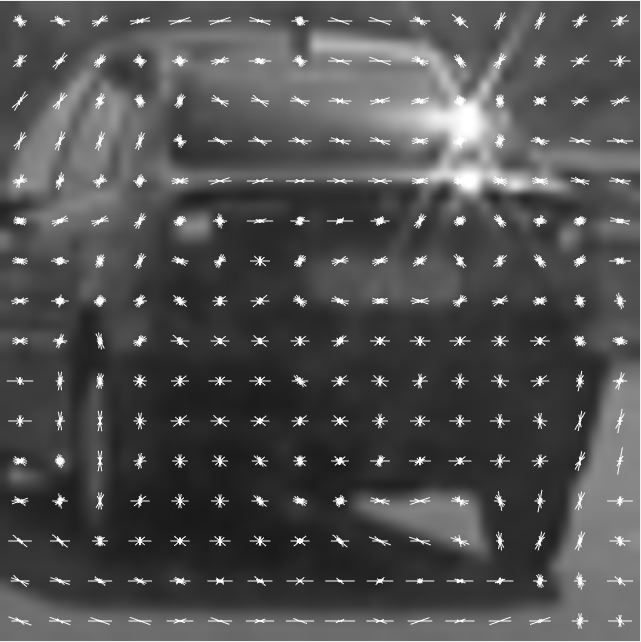
\includegraphics[width=7cm]{images/car_hog_gray4x4}
			\end{figure} \\
			\hline
		\end{tabular}
	\end{adjustbox}
	\captionof{figure}{Visualisasi Fitur HOG dengan ukuran sel 4 x 4 piksel}
	\label{fig:FiturHOG}
\end{table}

Untuk setiap piksel, hitung \textit{magnitude} gradien menggunakan persamaan \eqref{eqn:BesarGradien} dan arah gradien menggunakan persamaan \eqref{eqn:ArahGradien}.

\begin{equation*}
M(2,5) = \sqrt{0^2 + (-37)^2} = 37
\end{equation*}
\begin{equation*}
\theta(2,5) = arctan\frac{-37}{0} = 90
\end{equation*}

Setelah itu, tentukan ukuran sel, ukuran blok dan jumlah \textit{bins}. Pada awalnya, ukuran sel akan dipilih sebesar 2 $\times$ 2 piksel dan ukuran blok sebesar 2 kali lipat daripada ukuran sel yaitu 4 $\times$ 4 piksel. Lakukan perhitungan \textit{Histogram of Oriented Gradient} untuk semua sel dengan melakukan \textit{voting} arah gradien berdasarkan  \textit{magnitude} gradien, dimana arah gradien akan menjadi jumlah sudut \textit{bin}, dan \textit{magnitude} gradien akan menjadi bobot nilai yang kemudian dimasukkan berdasarkan persentase. Untuk contoh perhitungan analisis kali ini jumlah \textit{bins} yang dipakai sebanyak 9 buah, sehingga didapat nilai sudut setiap \textit{histogram bin} yaitu 180 / 4 = 45. Berikut merupakan contoh proses \textit{voting} untuk piksel dengan koordinat (2,5).

\begin{equation*}
M(2,5) = 37
\end{equation*}
\begin{equation*}
\theta(2,5) = 90
\end{equation*}

Sehingga untuk \textit{bin} dengan sudut 90 akan mendapat nilai bobot sebesar 37 yang didapatkan dari nilai gradien \textit{magnitude}-nya. Lakukan proses tersebut untuk setiap sel sampai setiap sel akan mempunyai \textit{Histogram of Oriented Gradient}. Kemudian untuk setiap blok akan dilakukan normalisasi dengan menggabungkan hasil histogram dari setiap sel dalam bloknya. Adapun proses normalisasi dapat menggunakan 4 algoritme yaitu, \textit{L1-Norm}, \textit{L1-Sqrt}, \textit{L2-Norm}, dan \textit{L2-Hys}. Penelitian ini akan menggunakan algoritme normalisasi \textit{L2-Norm} karena berdasarkan penelitian sebelumnya, hasil yang didapat lebih baik dari algoritme lainnya \cite{prahara}. Di bawah adalah contoh perhitungan normalisasi untuk blok pertama:
\begin{table}[H]
	\centering
	\begin{small}
		\begin{tabular}{|p{1cm}|p{1cm}|p{1cm}|p{1cm}|p{1cm}|p{1cm}|p{1cm}|p{1cm}|}
			\hline
			1 & 0 & 4 & 0 \\
			\hline
			0 & 0.76 & 36.24 & 0 \\
			\hline
			0 & 0 & 40 & 0 \\
			\hline
			0 & 1.65 & 36.35 & 0 \\
			\hline
		\end{tabular}
	\end{small}
	\captionof{figure}{Matriks hasil Perhitungan Histogram untuk seluruh sel\\}
	\label{fig:MatriksHasilPerhitunganHistogram}
\end{table}

Berdasarkan matriks pada gambar \ref{fig:MatriksHasilPerhitunganHistogram}. Elemen matriks yang akan kita gunakan dalam perhitungan normalisasi ini adalah seluruh elemen baris pertama dan baris kedua.

\begin{equation*}
L2_{Norm} = \sqrt{1^2 + 0^2 + 4^2 + 0^2 + \ldots + 36.5^2 + 0^2} = 51,360978379
\end{equation*}

Setiap nilai pada histogram dari sel dalam blok tersebut akan dibagi dengan nilai hasil normalisasinya. Berikut merupakan contoh matriks hasil perhitungan histogram baris pertama kolom 1-4.
\begin{gather*}
\begin{bmatrix}
0,019470034 & 0 & 0,077880136 & 0 \\
\end{bmatrix}
\end{gather*}

Lakukan proses normalisasi untuk setiap blok dengan menggeser secara horizontal sejauh 1 kali ukuran sel (setengah ukuran blok) dan kemudian secara vertikal sejauh 1 kali ukuran sel sa mpai blok tersebut sudah berada pada akhir dari bagian citra. Kemudian hasil dari proses normalisasi akan disusun menjadi matriks dengan kolom sebesar  \textit{jumlah bin} $\times$ \textit{lebar blok dalam satuan sel} $\times$ \textit{jumlah pergeseran horizontal} dan jumlah baris sebesar \textit{jumlah pergeseran vertikal} $\times$ \textit{tinggi blok dalam satuan sel} , dengan perhitungan tersebut, dalam analisa saat ini didapatkan ukuran matriks sebesar 6 $\times$ 8. Dalam analisa ini, hasil keluaran dari metode \textit{Histogram of Oriented Gradient} ada sebanyak 48 fitur. Matriks inilah yang akan dijadikan sebagai masukan bagi metode \textit{Machine Learning} yang akan digunakan dalam penelitian ini.\\

\subsection{\textit{Support Vector Machine}}
\textit{HOG descriptor} yang dihasilkan dari perhitungan metode \textit{Histogram of Oriented Gradient} akan digunakan sebagai bahan masukan \textit{Support Vector Machine}. Masukkan untuk metode SVM ini berupa matriks fitur berukuran jumlah data x jumlah data. \textit{Support Vector Machine} yang akan digunakan dalam penelitian ini akan menggunakan \textit{library} dari Weka SVM. \textit{Support Vector Machine} termasuk dalam algoritme \textit{supervised learning}. Konsep dasar dari metode ini adalah untuk menemukan sebuah \textit{separating hyperplane} (bidang) yang dapat memisahkan dua kelas sebagai keputusan klasifikasi. Dalam penelitian ini mobil yang akan dikenali adalah semua jenis mobil dari arah kiri dan kanan.

\begin{small}
	\begin{longtable}{| p {0.75cm} | p {0.7cm} | p {0.7cm} | p {0.7cm} | p {0.7cm} | p {0.7cm} | p {0.7cm} |  p {0.7cm} | p {0.7cm} | p {0.7cm} | p {0.7cm} | p {0.7cm} | p {0.7cm} | p {0.7cm} |}
		\caption{Tabel Contoh Data Latih} \\
		\hline
		\textbf{Data}  & \textbf{f1}  & \textbf{f2}  & \textbf{f3} & \textbf{f4} & \textbf{Class} \\
		\hline
		\endfirsthead
		\endhead
		\textbf{A1} & 5.1 & 3.5 & 1.4 & 0.2 & 1\\
		\hline
		\textbf{A2} & 4.9 & 3.0 & 1.4 & 0.2 & 1\\
		\hline
		\textbf{A3} & 7.0 & 3.2 & 4.7 & 1.4 & -1\\
		\hline
		\textbf{A4} & 6.4 & 3.2 & 4.5 & 1.5 & -1\\
		\hline
	\end{longtable}
\end{small}

Pada matriks fitur di atas, 1 menandakan kelas mobil dan -1 menandakan kelas bukan mobil. Berdasarkan matriks fitur tersebut, akan dibuat matriks RBF dengan ukuran sebanyak data. Misal terdapat 4 data yang digunakan maka ukuran matriks RBF adalah $4\times4$. Matriks RBF digunakan untuk menghitung \textit{dot product} dari masing-masing data. Pada perhitungan ini nilai $\sigma$ yang digunakan adalah 1.\\
\\
K(A1,A1) = $\exp(-\frac{|A1-A1|^2}{2\sigma^2})$
$=\exp(-\frac{|5.1-5.1|^2+|3.5-3.5|^2+|1.4-1.4|^2
+|0.2-0.2|^2}{2(1)^2})$\\
$=1$
\\\\
K(A1,A2) = $\exp(-\frac{|A1-A2|^2}{2\sigma^2})$
$=\exp(-\frac{|5.1-4.9|^2+|3.5-3.0|^2+|1.4-1.4|^2
	+|0.2-0.2|^2}{2(1)^2})$\\
$=0.8650222931107414$
\\\\
K(A1,A3) = $\exp(-\frac{|A1-A3|^2}{2\sigma^2})$
$=\exp(-\frac{|5.1-7.0|^2+|3.5-3.2|^2+|1.4-4.7|^2
	+|0.2-1.4|^2}{2(1)^2})$\\
$=3.3046824003738314E^{-4}$
\\\\
K(A1,A4) = $\exp(-\frac{|A1-A4|^2}{2\sigma^2})$
$=\exp(-\frac{|5.1-6.4|^2+|3.5-3.2|^2+|1.4-4.5|^2
	+|0.2-1.5|^2}{2(1)^2})$\\
$=0.001444488499020542$
\\\\
Dari perhitungan \textit{dot product} di atas maka akan terbentuk matriks RBF seperti pada tabel 3.4.
\begin{small}
	\begin{longtable}{| p {2cm} | p {2cm} | p {2cm} | p {2cm} | p {2cm} |}
		\caption{Tabel Perhitungan Matriks RBF} \\
		\hline
		\textbf{}  & \textbf{A1}  & \textbf{A2}  & \textbf{A3} & \textbf{A4} \\
		\hline
		\endfirsthead
		\endhead	
		\textbf{A1}&1 & 0.865022293	& 3.30E-4 &	1.44E-03\\
		\hline
		\textbf{A2}& 0.865022293 & 1 & 2.27E-4 & 1.11E-03\\
		\hline
		\textbf{A3}& 3.30E-4 & 2.27E-4 & 1	& 0.814647316\\
		\hline
		\textbf{A4}& 1.44E-03 & 1.11E-03 & 0.814647316 & 1\\
		\hline
		\hline
		
	\end{longtable}
\end{small}

Setelah mendapatkan matriks RBF, maka dapat membuat persamaan linear untuk mendapatkan nilai $\alpha$ dan $b$ (bias) berdasarkan persamaan \textit{hyperplane} SVM yaitu persamaan \ref{eqn:rbfkernel}.\\
Contoh perhitungan:\\
$(1)\alpha_1 + (1)\alpha_2 + (-1)\alpha_3 + (-1)\alpha_4 + (0)b = 0$\\
$(1)\alpha_1 + (0.865022293)\alpha_2 + (-3.30E^{-4})\alpha_3 + (-1.44E^{-3})\alpha_4 + b = 1$\\
$(0.865022293)\alpha_1 + (1)\alpha_2 + (-2.27E^{-4})\alpha_3 + (-1.11E^{-3})\alpha_4 + b = 1$\\
$(3.30E^{-4})\alpha_1 + (2.27E^{-4})\alpha_2 + (-1)\alpha_3 + (-0.814647316)\alpha_4 + b = -1$\\
$(1.44E^{-3})\alpha_1 + (1.11E^{-3})\alpha_2 + (-0.814647316)\alpha_3 + (-1)\alpha_4 + b = -1$\\

Untuk mendapatkan solusi ($\alpha_1, \alpha_2, \alpha_3, \alpha_4, b$) dari sistem persamaan linear di atas dapat menggunakan \textit{library} JAMA. Berikut adalah solusi yang diperoleh dari sistem persamaan di atas.
\begin{small}
	\begin{longtable}{| p {2cm} | p {2cm} | p {2cm} | p {2cm} | p {2cm} |}
		\caption{Tabel nilai $\alpha$ dan $b$} \\
		\hline
		$\alpha_1$  & $\alpha_2$  & $\alpha_3$ & $\alpha_4$ & $b$ \\
		\hline
		\endfirsthead
		\endhead
		0.544855 & 0.543123 & 0.541044 & 0.546933 & -0.013700\\
		\hline
		
	\end{longtable}
\end{small}

Nilai $\alpha$ dan $b$ yang telah diperoleh kemudian disimpan untuk keperluan proses klasifikasi. Misal terdapat data uji sebagai berikut:
\begin{small}
	\begin{longtable}{| p {0.75cm} | p {0.7cm} | p {0.7cm} | p {0.7cm} | p {0.7cm} | p {0.7cm} | p {0.7cm} |  p {0.7cm} | p {0.7cm} | p {0.7cm} | p {0.7cm} | p {0.7cm} | p {0.7cm} | p {0.7cm} |}
		\caption{Tabel Contoh Data Uji} \\
		\hline
		\textbf{Data}  & \textbf{f1}  & \textbf{f2}  & \textbf{f3} & \textbf{f4} & \textbf{Class} \\
		\hline
		\endfirsthead
		\endhead
		\textbf{T1} & 4.6 & 3.1 & 1.5 & 0.2 & ?\\
		\hline
	\end{longtable}
\end{small}
Dalam proses pengujian, langkah yang ditempuh mirip dengan proses pelatihan. Pertama adalah membentuk matriks RBF untuk pengujian dengan menggunakan data latih pada tabel 3.3. Contoh perhitungan adalah sebagai berikut:\\\\
K(T1,A1) = $\exp(-\frac{|T1-A1|^2}{2\sigma^2})$
$=\exp(-\frac{|4.6-5.1|^2+|3.1-3.5|^2+|1.5-1.4|^2
	+|0.2-0.2|^2}{2(1)^2})$\\
$=0.8105842459701871$
\\\\
K(T1,A2) = $\exp(-\frac{|T1-A2|^2}{2\sigma^2})$
$=\exp(-\frac{|4.6-4.9|^2+|3.1-3.0|^2+|1.5-1.4|^2
	+|0.2-0.2|^2}{2(1)^2})$\\
$=0.9464851479534836$
\\\\
K(T1,A3) = $\exp(-\frac{|T1-A3|^2}{2\sigma^2})$
$=\exp(-\frac{|4.6-7.0|^2+|3.1-3.2|^2+|1.5-4.7|^2
	+|0.2-1.4|^2}{2(1)^2})$\\
$=1.6247279265951668E^{-4}$
\\\\
K(T1,A4) = $\exp(-\frac{|T1-A4|^2}{2\sigma^2})$
$=\exp(-\frac{|4.6-6.4|^2+|3.1-3.2|^2+|1.5-4.5|^2
	+|0.2-1.5|^2}{2(1)^2})$\\
$=9.396529058360945E^{-4}$
\\\\
Dari perhitungan \textit{dot product} maka akan terbentuk matriks RBF uji seperti pada tabel 3.7 di bawah ini.
\begin{small}
	\begin{longtable}{| p {2cm} | p {2cm} | p {2cm} | p {2cm} | p {2cm} |}
		\caption{Tabel Perhitungan Matriks RBF Uji} \\
		\hline
		\textbf{}  & \textbf{A1}  & \textbf{A2}  & \textbf{A3} & \textbf{A4} \\
		\hline
		\endfirsthead
		\endhead	
		\textbf{T1} & 0.810584245 & 0.946485147 & 1.62E-4 & 9.39E-4
		\\
		\hline	
	\end{longtable}
\end{small}
Setelah mendapatkan matriks RBF uji maka proses klasifikasi dapat dilakukan dengan menggunakan persamaan 2.15. Perhitungan klasifikasi adalah sebagai berikut:\\\\
$f(x) = sign[(0.810584 * 0.810584245  * 1.0) + (0.946485 * 0.946485147 * 1.0) + (1.624727 * 1.62E^{-4} * (-1.0)) + (9.396529 * 9.396529058E^{-4} * (-1.0)) + (-0.013700) ]$\\
$=1$

Setelah dilakukannya perhitungan manual antara data uji terhadap data latih, nilai yang diperoleh adalah 1 yang artinya data uji masuk ke dalam kelas 1 (positif). Jika hasil perhitungan bernilai -1 maka data uji masuk ke dalam kelas -1 (negatif). Misal dalam pengujian di atas kelas 1 adalah mobil dan kelas -1 adalah bukan mobil, maka data uji tergolong kelas mobil.
\newpage